\documentclass[11pt]{article}
\usepackage[english]{babel}
\usepackage{geometry}
\usepackage{amsmath}
\usepackage{amsthm}
\usepackage{graphicx}
\usepackage[utf8]{inputenc}

%%%%%%%% MARGIN
\geometry{verbose, letterpaper, tmargin=3cm,
  bmargin=3cm,lmargin=2.5cm,rmargin=2.5cm}

%%%%%%%% NO PARAGRAPH INDENT
% https://tex.stackexchange.com/questions/27802/set-noindent-for-entire-file
\setlength\parindent{0pt}

%%%%%%%% SUB-FIGURE PACKAGE
\usepackage{subcaption}

%%%%%%%% HYPERREF PACKAGE
\usepackage{hyperref}
\hypersetup{linkcolor=blue}
\hypersetup{citecolor=blue}
\hypersetup{urlcolor=blue}
\hypersetup{colorlinks=true}

%%%%%%%% DEFINITION AND THEOREM DEFINITIONS
\theoremstyle{definition}
\newtheorem{definition}{Definition}[section]

\theoremstyle{remark}
\newtheorem{remark}{Remark}

\theoremstyle{remark}
\newtheorem{question}{Question}

\newtheorem{theorem}{Theorem}[section]

%%%%%%%% MULTI-COLUMNS PACKAGE
\usepackage{multicol}

%%%%%%%% BIB-LATEX STUFF
\usepackage[style=numeric,
            bibstyle=numeric,
            citestyle=numeric,
            hyperref=true,
            backend=biber]{biblatex}
\addbibresource{ref.bib} %Put relative path to ref

%%%%%%%% SETS DEFINITIONS
\usepackage{amssymb}
%%%% Important sets
\renewcommand{\O}{\mathbb{O}}
\newcommand{\N}{\mathbb{N}}
\newcommand{\Z}{{\mathbb{Z}}}
\newcommand{\Q}{{\mathbb{Q}}}
\newcommand{\R}{{\mathbb{R}}}

%%%% Statistics
\newcommand{\E}[1]{\mathbb{E}\left[#1 \right]}
\newcommand{\V}[1]{\mathrm{Var}\left[#1 \right]}
\renewcommand{\P}[1]{\mathrm{P}\left(#1 \right)}

%%%% Lambda Calculus Symbols
\newcommand{\dneq}{\,\, \# \,\,}
\renewcommand{\S}{\pmb{\mathrm{S}}}
\newcommand{\I}{\pmb{\mathrm{I}}}
\newcommand{\K}{\pmb{\mathrm{K}}}
\newcommand{\ch}[1]{\ulcorner #1 \urcorner}

%%%% Ordinal Lambda Calculus Symbols
\newcommand{\ordAlph}{\Sigma_{\text{Ord}}}
\newcommand{\termOrd}{\text{Term}_\text{Ord}}
\newcommand{\fl}{\mathrm{fl}}
\newcommand{\sk}{\mathrm{sk}}

%%%% Superscript to the left
% https://latex.org/forum/viewtopic.php?t=455
\usepackage{tensor}
\newcommand{\app}[3]{\tensor*[^{#1}]{\left(#2, #3\right)}{}}

%%%% Make optional parameter
% https://tex.stackexchange.com/questions/217757/special-behavior-if-optional-argument-is-not-passed
\usepackage{xparse}
\NewDocumentCommand{\cx}{o}{
  \IfNoValueTF{#1}
  {\left[\quad\right]}
  {\left[\, #1 \,\right]}
}

%%%%%%%% LOGIC TREES
\usepackage{prftree}

%%%%%%%% SPLIT EQUATIONS
% https://tex.stackexchange.com/questions/51682/is-it-possible-to-pagebreak-aligned-equations
\allowdisplaybreaks

%%%%%%%% FLOAT SPECIFIER
% https://www.overleaf.com/learn/latex/Errors/LaTeX_Error:_Unknown_float_option_%60H%27
\usepackage{float}

%%%%%%%% ENUMERATE LABEL
% https://www.latex-tutorial.com/tutorials/lists/
\usepackage{enumitem}

%%%%%%%% CODE RENDERING !!! UNCOMMENT IF NEEDED !!!
% Compile with flag -shell-escape
%\usepackage{minted}

%%%%%%%% START DOCUMENT

\title{Non-Parametric Statistics Workshop 1}
\author{David Plazas Escudero \\
  Juan Pablo Vidal \\
  Juan Sebasti\'an C\'ardenas-Rodríguez \\
  \scalebox{0.7}{Mathematical Engineering, Universidad EAFIT}}
\date{\today}


\begin{document}
\maketitle
\section{Workshop Exercises}
The code done to solve this workshop can be found in a Jupyter
notebook in \href{https://bit.ly/2SNMPod}{this link}.
\subsection*{Exercise 1}
The data used is the average daily temperatures in Canada for the past
35 years. The empirical cumulative distributions (ECDFs) for each year
are presented in Figure \ref{fig:ecdfs_temps}, where the yellow-most
curve represents the ECDF of the data recorded for the first year, and
the blue-most is the last year.
\begin{figure}[H]
    \centering
    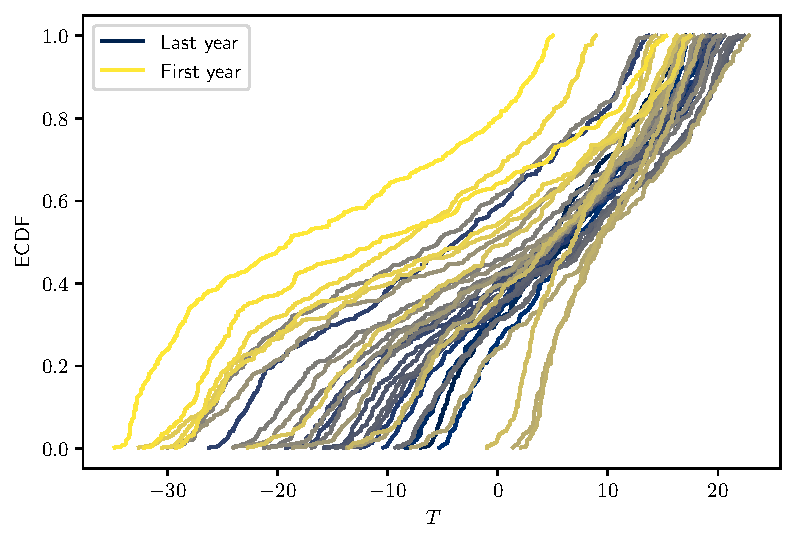
\includegraphics[scale=.5]{../figs/ecdfs.pdf}
    \caption{Empirical distributions by years.}
    \label{fig:ecdfs_temps}
\end{figure}

Based on this plots, it can be observed a climate change effect over
the years. The plots of the first years arise for lower values of the
temperature $T$, whereas the last years tend to be on the right of the
plot. This can be interpreted as follows: since the plots for the
early years are on the left, these years reported more data on lower
average daily temperature than the most recent years. This means that
recent years have been hotter in average daily temperature.

\subsection*{Exercise 2}

The plug-in principle is a technique used in probability theory and
statistics to estimate a parameter of a probability distribution (e.g.,
the expected value, the variance, a quantile) that cannot be exactly computed.
In general, the plug-in principle says that a feature of a
given distribution can be approximated by the same feature of the
empirical distribution of a sample of observations drawn from the
given distribution \cite{van2000asymptotic}.

The feature of the empirical distribution is called a plug-in estimate
of the feature of the given distribution. For example, a quantile of a
given distribution can be approximated by the analogous quantile of
the empirical distribution of a sample of draws from the given
distribution. The following is a formal definition of plug-in estimate.
\\

A statistical functional $T(F)$ is any function of $F$. The plug-in estimator of $\theta=T(F)$ is defined by

\[
  \widehat{\theta}_{n}=T\left(\widehat{F}_{n}\right)
\]

A functional of the form $\int a(x) d F(x)$ is called a linear
functional. The plug-in estimator for linear functional $T(F)=\int a(x) d F(x)$
is:

\[
  T\left(\widehat{F}_{n}\right)=\int a(x) d
  \widehat{F}_{n}(x)=\frac{1}{n} \sum_{i=1}^{n} a\left(X_{i}\right)
\]

It is important to note that $T\left(F_{n}\right)$ converges to $T(F)$
as the sample size $n$ increases.

In the practice, the limited area is calculated in the first quadrant
for each empirical curve of the temperature data, this allows to
extract the plug-in estimator of the mean, since the difference
between the area with positive values and the area with negative
values is extracted from the empirical curve, which allows estimating
the mean of the series. The plug-in estimation of the mean for each
year is presented in Figure \ref{fig:plug-in}, where a comparison with
the natural estimator of the mean is presented.


\begin{figure}[H]
    \centering
    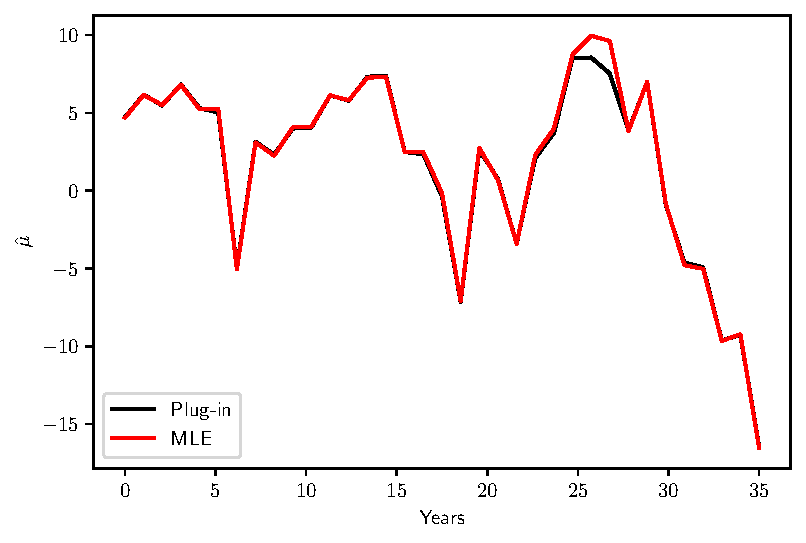
\includegraphics[scale=.5]{../figs/means.pdf}
    \caption{Mean estimation of the series.}
    \label{fig:plug-in}
\end{figure}

From Figure \ref{fig:plug-in}, an almost identical estimation can be seen
between the two estimators, however it shows
a slight difference between the mean estimates, this is because the
only case in which both estimates are identical is when the sample
size is infinite.


\begin{figure}[H]
    \centering
    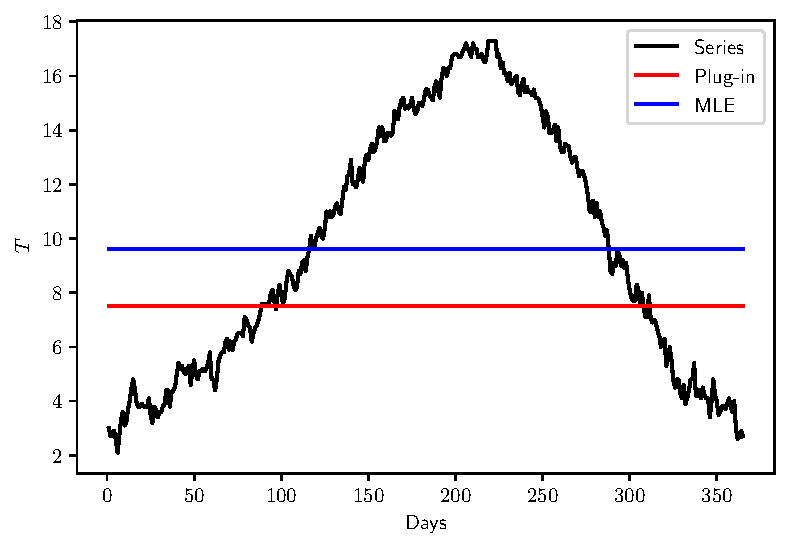
\includegraphics[scale=.5]{../figs/mle-vs-plugin.pdf}
    \caption{Comparison between the natural estimator and the plug-in estimator.}
    \label{fig:comparision}
\end{figure}

\subsection*{Exercise 3}
Calculate and plot the confidence bands for the empirical continuous
distribution function (ECDF) of the coldest and hottest year in
average with a confidence of 95 \% . Are there any sectors that are
not enclosed in the bands?

\begin{proof}
  Let $n$ be the size of the sample and $1 - \alpha$ the desired
  confidence for the bands. This method is based on the
  Dvoretzky–Kiefer–Wolfowitz inquality (see \cite{wasserman2006}).
  In order to calculate the confidence bands for the
  ECDF, we first define $\epsilon_n$ by the following formula:
  \begin{equation*}
    \epsilon_n = \sqrt{\frac{1}{2n} \ln\left(\frac{2}{\alpha}\right)}
  \end{equation*}

  Let $\hat{F}_n(x)$ be the ECDF. Then, for each $x$ in the ECDF we
  define the lower ($L(\cdot)$) and upper ($U(\cdot)$) bound by:
  \begin{align*}
    L(x) &= \max\{\hat{F}_n(x) - \epsilon_n, 0\} \\
    U(x) &= \min\{\hat{F}_n(x) + \epsilon_n, 1\}
  \end{align*}

  The results obtained by using the temperatures of the coldest and
  hottest year are seen in Figure \ref{fig:ex3}.
  \begin{figure}[H]
    \centering
    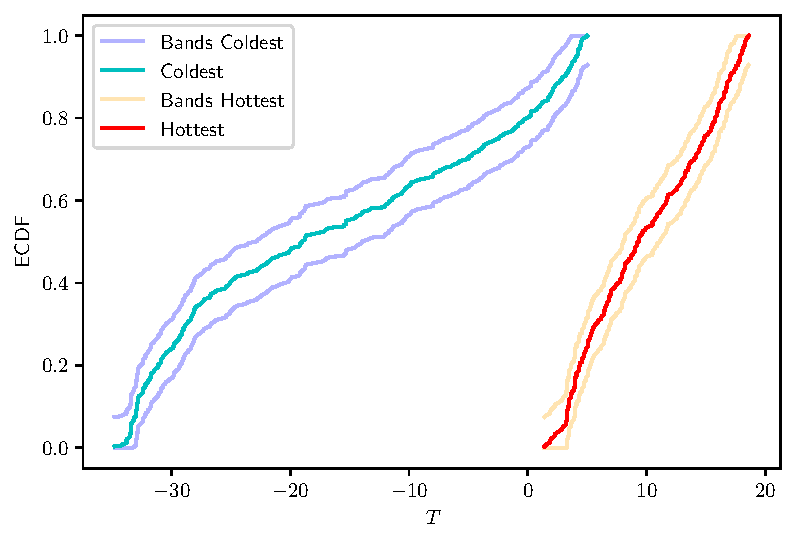
\includegraphics[scale=0.5]{../figs/ecdf_bands.pdf}
    \caption{Bands for the coldest and hottest year.}
    \label{fig:ex3}
  \end{figure}

  It can be seen that the upper and lower bands fully enclose the
  ECDF. Nevertheless, there exists two points where the function and
  the bands meets. This happens in the lower band at the beginning and
  the upper band at the final point.

  This phenomenon is due to the full certainty at those points in a
  sense that the lower bound, at the start, has to be the same point
  as it cannot go lower than 0. A similar reasoning can explain the
  upper bound and the final point.
\end{proof}

\subsection*{Exercise 4}
Write and execute a code that allows to visualize the Glivenko
Cantelli for a Weibull distribution.
\begin{proof}
  The Glivenko Cantelli shows the relationship of how the difference
  between the empirical and theoretical distribution changes depending
  of the number of the sample.

  In this manner, if $n$ is the size of the sample, $\hat{F}_n(\cdot)$ is
  the ECDF of that sample and $F(\cdot)$ is the theoretical distribution
  the theorem states that:
  \begin{equation*}
    \sup_x \mid \hat{F_n}(x) - F(x) \mid \xrightarrow[]{\text{a.s.}} 0.
  \end{equation*}
  We generated Weibull random variables of different
  sizes $n_i$ calculated with:
  \begin{equation*}
    n_i = 2^i, \quad \text{for } i=1,\ldots,20
  \end{equation*}
  The results of the experiment can be found in Figure \ref{fig:ex4}.
  \begin{figure}[H]
    \centering
    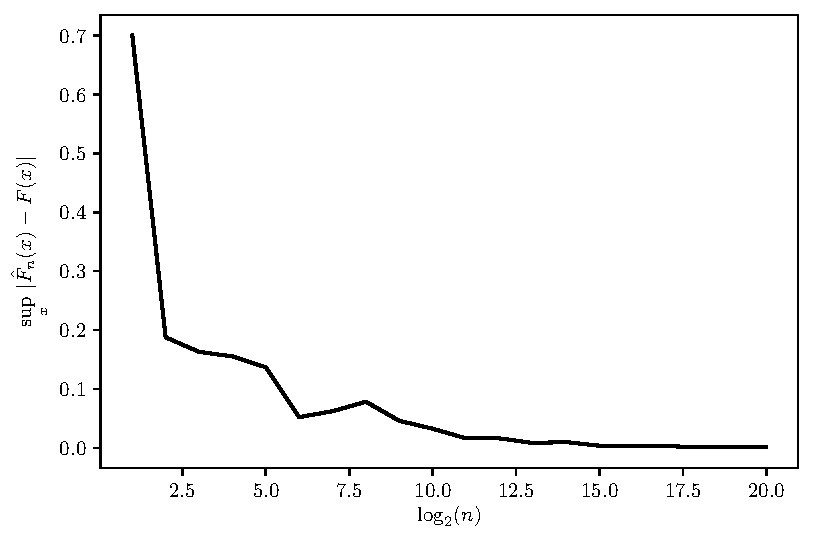
\includegraphics[scale=0.5]{../figs/weibull.pdf}
    \caption{Glivenko Cantelli theorem visualization.}
    \label{fig:ex4}
  \end{figure}

  It is clear that the biggest difference between the ECDF and the
  theoretical distribution starts to go to 0 when $n$ gets
  bigger. Furthermore, although the behavior in the graph does not
  show a monotone decrease, it does display the asymptotic behavior
  described in the theorem.
\end{proof}

\subsection*{Exercise 5}
\begin{theorem}[Jensen's Inequality]
  Let $g(\cdot)$ be a concave function and let $X$ be a random
  variable, then
\[
  \E{g(X)} \leq g(\E{X}).
\]
\end{theorem}

\begin{proof}
  Let $g(\cdot)$ be a concave function and $L(x)$ be its tangent line
  at a fixed point $x_0$. It holds that (see Theorem 6 from
  \cite{nachbar2018concave})
\begin{equation}\label{eq:conc}
  g(x) \leq L(x).
\end{equation}
If $x_0=\E{X}$. From (\ref{eq:conc}) and given that $\E{\cdot}$
preserves order, we have
\[
  \E{g(X)} \leq \E{L(X)} = \E{a+bX} = a + b\E{X} = L(\E{X}) =
  g(\E{X}).
\]
\end{proof}

\subsection{Exercise 6}

\subsubsection*{ L-estimator }

An L-estimator is  a linear combination of order statistics of the measurements,
often called L-statistic. They have the
advantage of being robust and simple to use, but tend to have problems
with low efficiency. Not all L-estimators are robust (for example, the
minimum, maximum and mean are not considered robust) and some have
better efficiency than others. L-statistics with multiple (correct)
weights will tend to be more efficient than those with fewer weights
or poorly chosen weights \cite{andersen2008modern}.

L-estimators for a sample size n are defined by $T_n$:

\begin{align*}
  &T_{n}\left(X_{1}, \ldots, X_{n}\right)=\sum_{i=1}^{n} a_{i} X_{n,(i)}\\
  &a_{i}=\int_{(i-1) / n}^{i / n} h(x) \mathrm{d} x, \quad
  \int_{0}^{1} h(x) \mathrm{d} x=1
\end{align*}

where: $X_{n}$ are the order statistics and $a_{i}$ are weight
factors.

L-estimators are useful in robust statistics, but they are
considered inefficient. In modern statistics M-estimators are
preferred, though these are much more difficult to implement computationally. In
many circumstances, L-estimators are reasonably easier to implement and, thus,
adequate for initial estimation. M-estimators provide robust
statistics that also have high relative efficiency, at the cost of
being much more computationally complex \cite{andersen2008modern}.

\subsubsection*{Examples}

 \begin{figure}[H]
  \centering
  \begin{subfigure}[t]{0.475\textwidth}
      \centering
      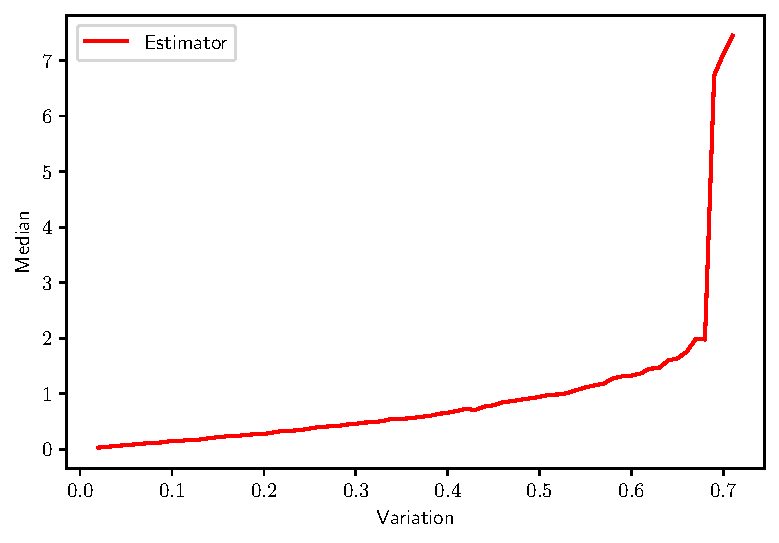
\includegraphics[scale=0.40]{../figs/median.pdf}
      \caption{Median estimator.}
  \end{subfigure}
  \begin{subfigure}[t]{0.475\textwidth}
      \centering
      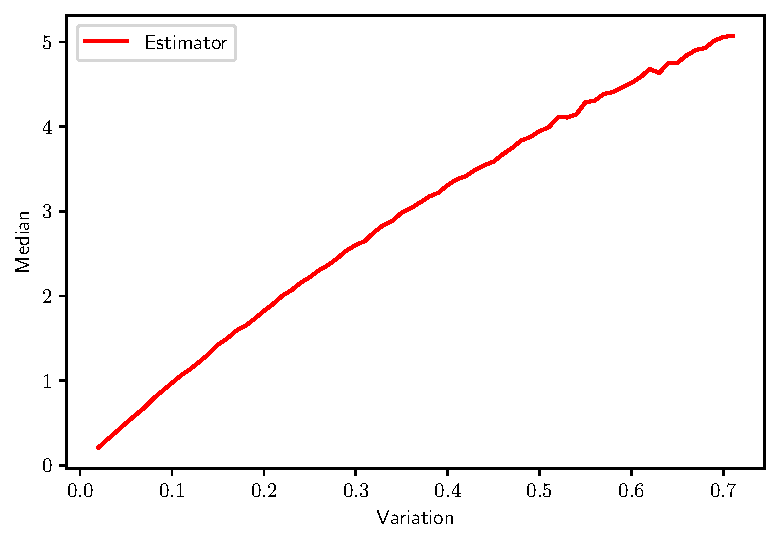
\includegraphics[scale=0.40]{../figs/mean-L.pdf}
      \caption{Mean estimator.}
  \end{subfigure}
  \caption{L-estimators.}
  \label{fig:L-Estimators_1}
\end{figure}

Figure \ref{fig:L-Estimators_1} shows the influence function of the
median and mean. It can be seen that the median is a much more robust
statistic, which maintains a high breakdown point, above 50\%, allowing the
estimator to remain unchanged when modifying or contaminating the
sample. In this case, random data is generated from a standard normal
distribution, and by contaminating the sample in multiple percentages,
the median remains with a very similar value until it exceeds the
breakdown point, which is 50\%, the highest in the L-estimators.

On the other hand, it can be seen that the mean, a measures of central
tendency, is a non-robust estimator, which varies according to how the
sample is modified, with a breakdown point of 1/N, since any change
modifies its value.

\begin{figure}[H]
  \centering
  \begin{subfigure}[t]{0.475\textwidth}
      \centering
      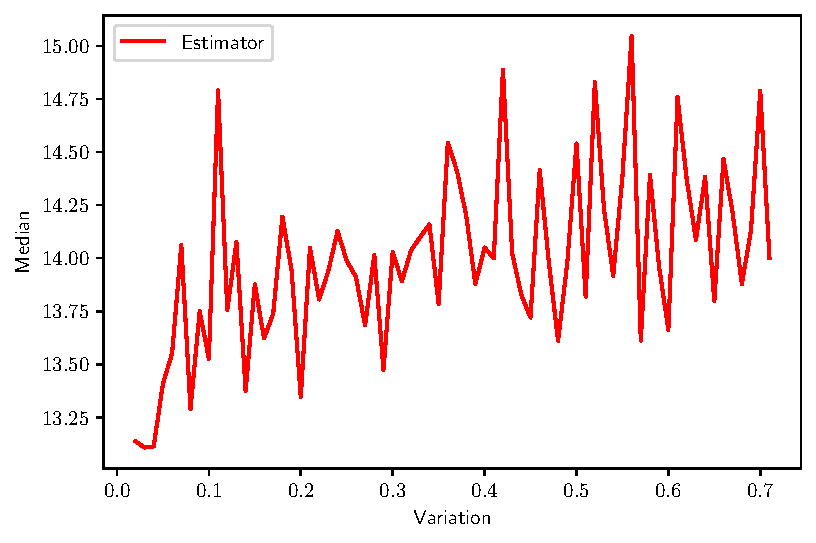
\includegraphics[scale=0.40]{../figs/max-L.pdf}
      \caption{Maximum estimator.}
  \end{subfigure}
  \begin{subfigure}[t]{0.475\textwidth}
      \centering
      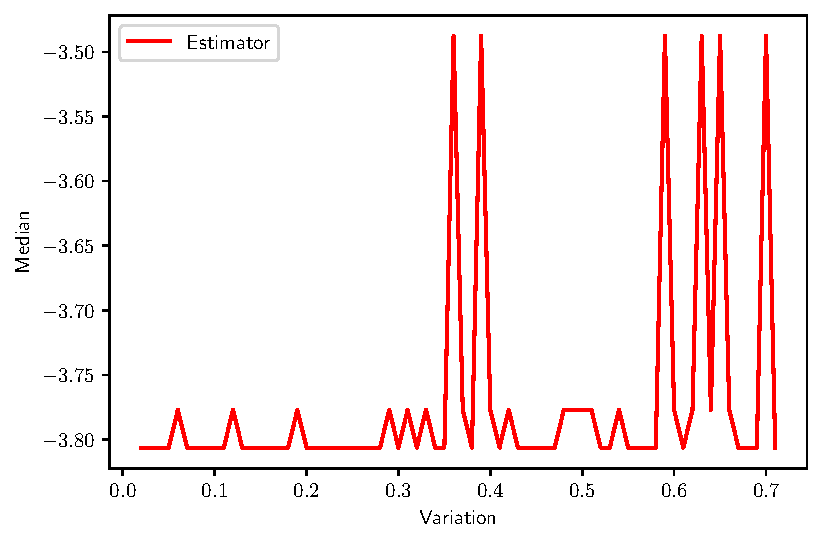
\includegraphics[scale=0.40]{../figs/min-L.pdf}
      \caption{Minimum estimator.}
  \end{subfigure}
  \caption{L-estimators.}
  \label{fig:L-Estimators_2}
\end{figure}

Figure \ref{fig:L-Estimators_2} shows the influence function of the
maximum and minimum, these non-robust estimators have a break down
point of 0, since any modification of the sample can alter its value
considerably, as can be seen in both figures, where in any percentage
of contamination, the estimator has a totally different value.

 \subsubsection*{M-estimator}

 M-estimators are a broad class of extremum estimators for which the
 objective function is a sample average \cite{andersen2008modern}. The
 extremum estimators are a wide class of estimators for parametric
 models that are calculated through maximization (or minimization) of
 a certain objective function. An M-estimator minimizes the function:

$$Q\left(e_{i}, \rho\right)=\sum_{i} \rho\left(\frac{e_{i}}{s}\right)$$

where $\rho$ is a symmetric function of the residuals

\begin{itemize}
\item The effect of $\rho$ is to reduce the influence of outliers
\item $s$ is an estimate of scale.
\item The robust estimates $\hat{\beta}$ are computed by the
  iteratively re-weighted least squares algorithm
\item We have several choices available for the weighting functions to
  be used
\end{itemize}

The M-estimator is more efficient under certain conditions: the data
contains y outliers and the model matrix is measured with no errors
\cite{susanti2014m}.

This estimators are especially useful when the data has outliers or is
contaminated by heavy tailed errors. On the
other hand, M-estimation is not recommended when anomalous data
reflects the true population, or the population is made up of distinct
mixture of distributions.

 \subsubsection*{Examples}

 \begin{figure}[H]
  \centering
  \begin{subfigure}[t]{0.475\textwidth}
      \centering
      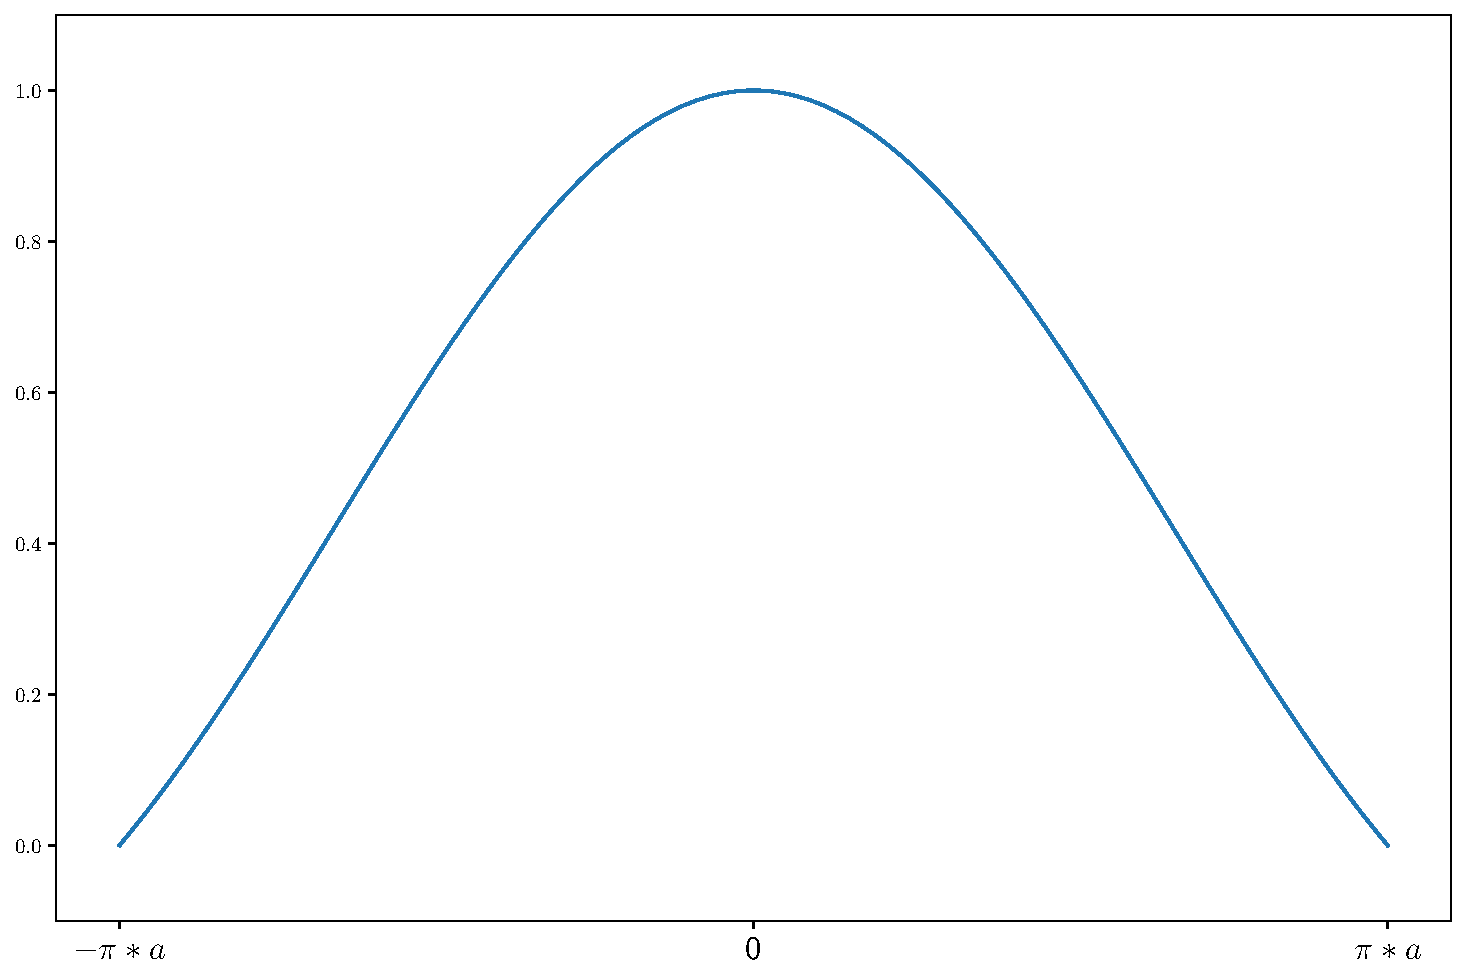
\includegraphics[scale=0.20]{../figs/AndrewWave.pdf}
      \caption{Andrew’s Wave estimator.}
  \end{subfigure}
  \begin{subfigure}[t]{0.475\textwidth}
      \centering
      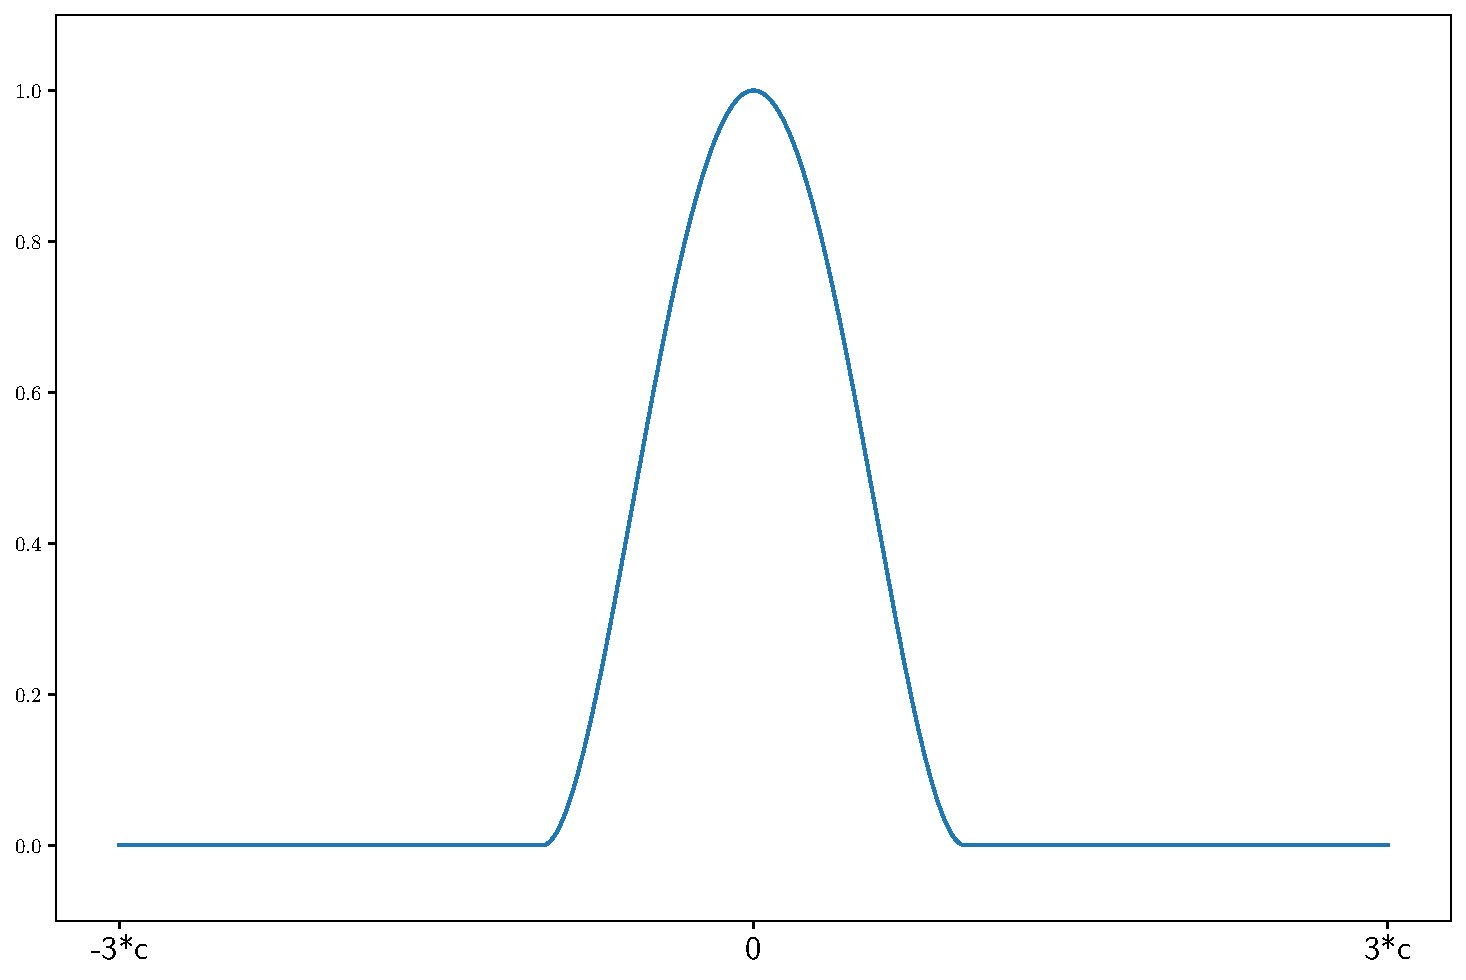
\includegraphics[scale=0.20]{../figs/TukeyBiweight.pdf}
      \caption{Tukey’s Biweight estimator.}
  \end{subfigure}
  \caption{M-estimators.}
  \label{fig:M-estimators_1}
\end{figure}

\begin{figure}[H]
  \centering
  \begin{subfigure}[t]{0.475\textwidth}
      \centering
      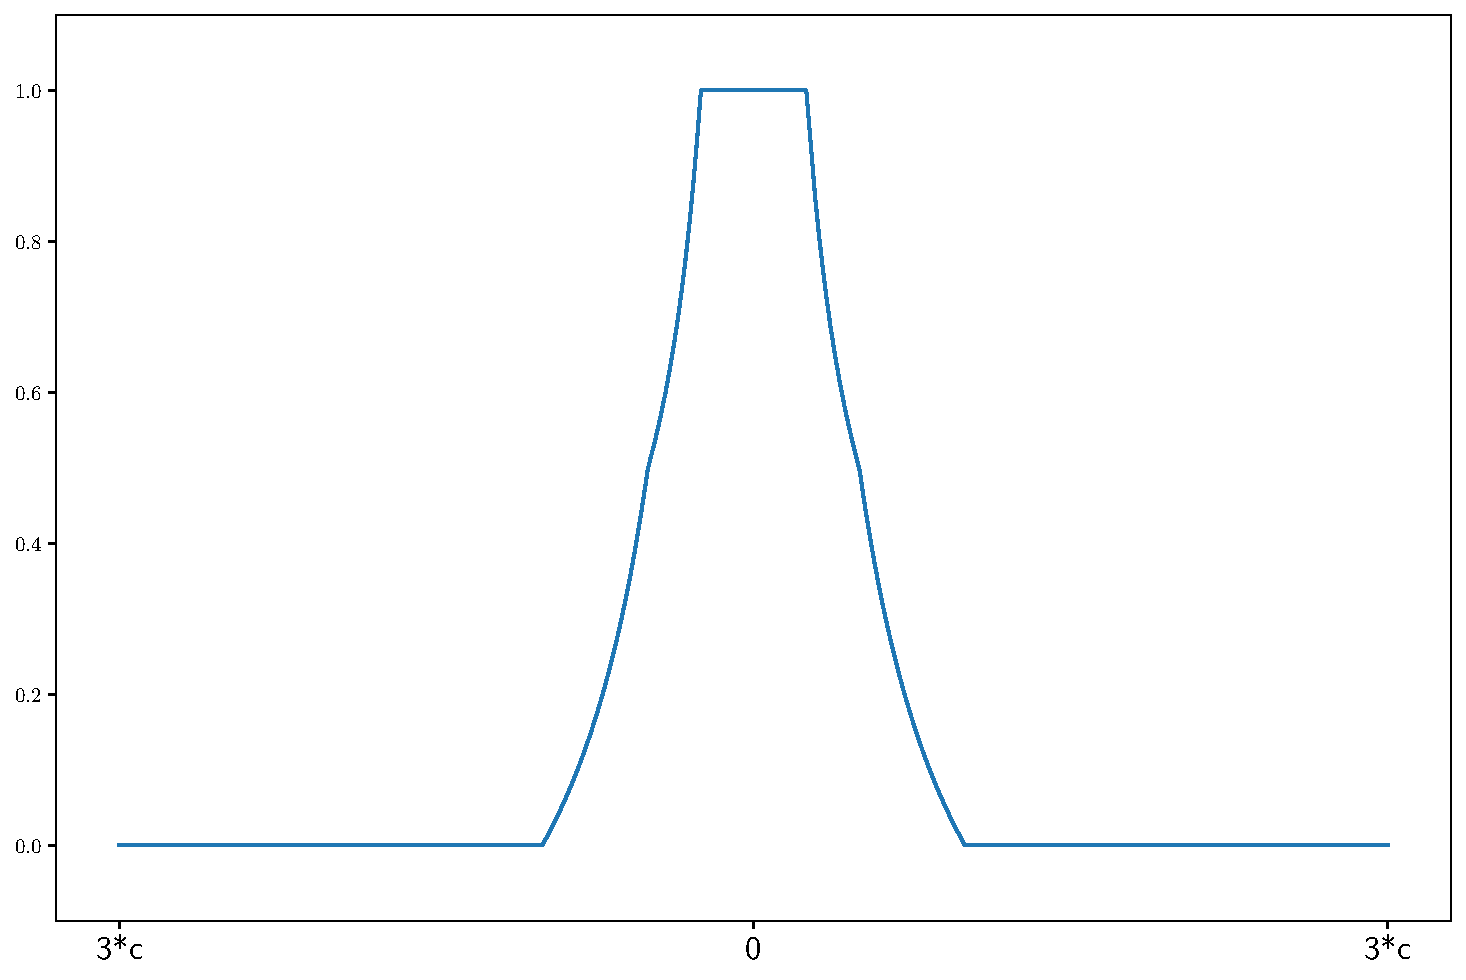
\includegraphics[scale=0.20]{../figs/Hampel.pdf}
      \caption{Hampel’s estimator.}
  \end{subfigure}
  \begin{subfigure}[t]{0.475\textwidth}
      \centering
      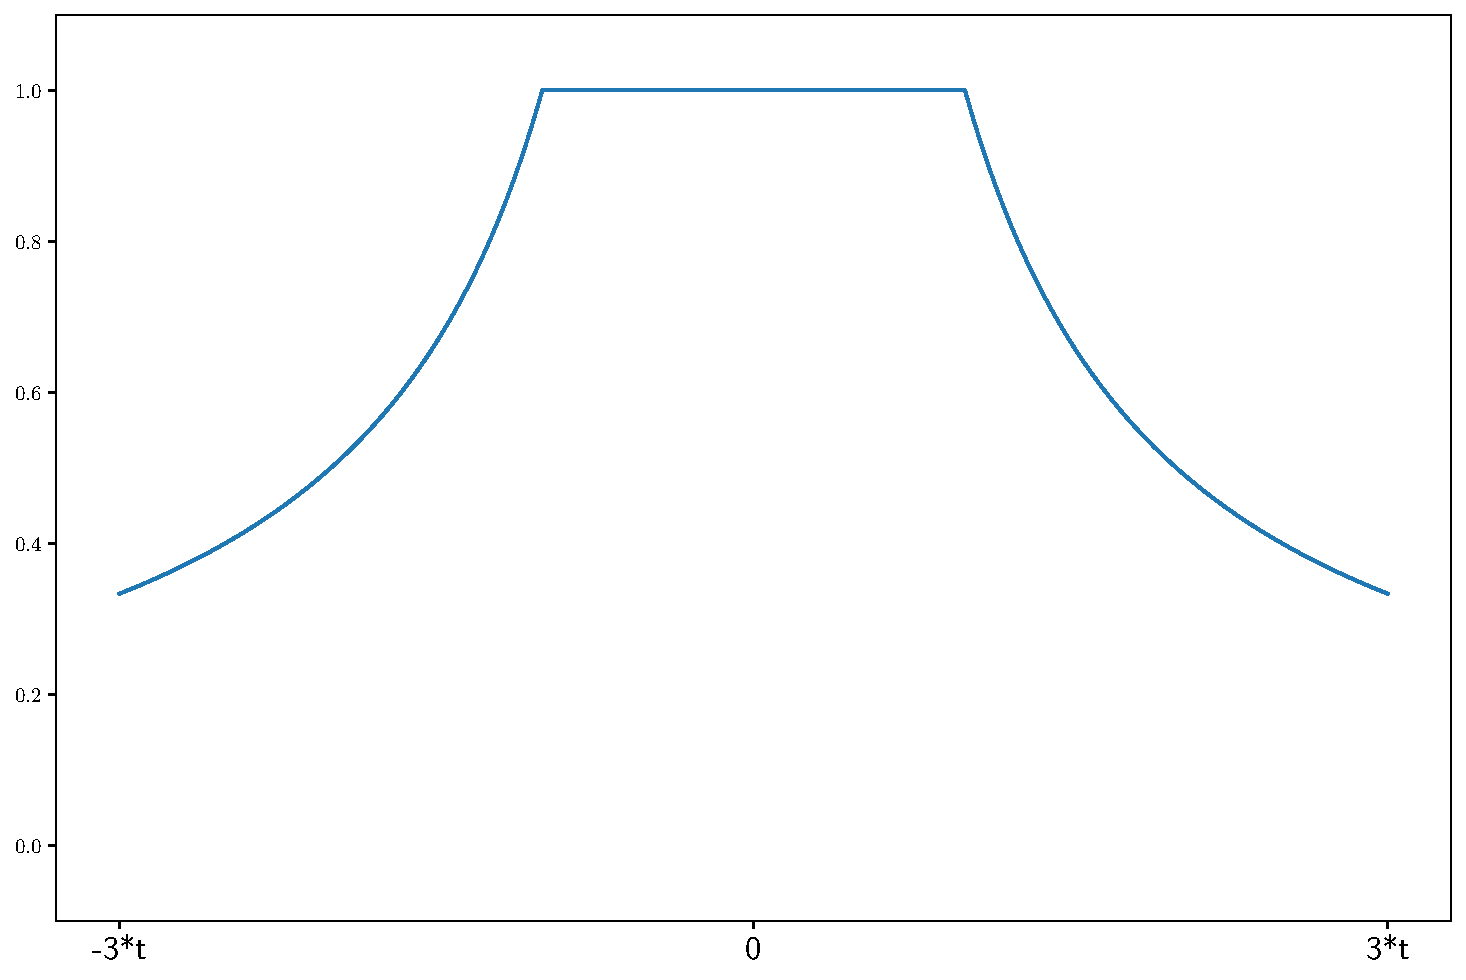
\includegraphics[scale=0.20]{../figs/HuberT.pdf}
      \caption{Huber’s T estimator.}
    \end{subfigure}
  \caption{M-estimators.}
  \label{fig:M-estimators_2}
\end{figure}

Figures \ref{fig:M-estimators_1} and Figure \ref{fig:M-estimators_2}
shows redescending M-estimators, which are estimators which have
functions that are non-decreasing near the origin, but decreasing
toward 0 far from the origin. These kinds of estimators are very
efficient, have a high breakdown point (close to 0.5) and, unlike
other outlier rejection techniques, they do not suffer from a masking
effect. They are efficient since they completely reject gross
outliers, and do not completely ignore moderately large outliers (like
median). In this case the worst estimator is Hubert T estimator,
because the other estimators completely reject gross outliers, while
the Huber estimator effectively treats these the same as moderate
outliers \cite{susanti2014m}.



\subsection*{Exercise 7}
\label{subsec:7}
Deduce the distribution and density of the $j$-th ordered
statistic. Explain with detail what would be a simple procedure to
simulate the $j$-th ordered statistic. Simulate 1000 observations of
some ordered statistic of a sample of size n that comes from a Weibull
distribution. Draw in a same graph the ECDF and theoretical
distribution.

\begin{proof}
  Let's first deduce the distribution and density of the $j$-th
  ($X_{[j]}$) ordered statistic. Let $X_1, \ldots, X_n$ be independent
  random variables that come from a distribution $F(\cdot)$. Hence,
  the probability that $X_i \le t$ is given by:
  \begin{equation*}
    \P{X_i \le t} = F(t)
  \end{equation*}
  Let $Z_t$ be a random variable that represents the number of
  variables whose value are less than $t$. Hence:
  \begin{equation*}
    Z_t \in \{0, 1, \ldots, n\}
  \end{equation*}
  Hence:
  \begin{align*}
    \P{Z_t = 0} &= \P{X_1 > t \wedge \ldots \wedge X_n>t} \\
                &= \P{X_1 > t} \ldots \P{X_n > t} \\
                &= (1 - F(t))\ldots (1 - F(t)) \\
                &= (1 - F(t))^n \\
    \P{Z_t = 1} &= \binom{n}{1} \P{X_1 \le t \wedge X_2 > t \wedge \ldots \wedge X_n > t} \\
                &=\binom{n}{1} F(t) (1 - F(t)) \ldots (1 - F(t)) \\
                &= \binom{n}{1} F(t) (1 - F(t))^{n-1} \\
                &\quad \vdots \\
    \P{Z_t = j} &= \binom{n}{j} F(t)^j (1 - F(t))^{n - j}
  \end{align*}
  Hence, the distribution $j$-th ordered statistic is given by:
  \begin{equation*}
    \label{eq:jth}
    \P{X_{[j]} \le t} = \P{Z_t \ge j} = \sum_{i=j}^n \binom{n}{i} F(t)^i (1 - F(t))^{n - i}
  \end{equation*}
  In these manner, we obtained the distribution for the $j$-th ordered
  statistic. Then, to obtain the density ($f_{[j]}(\cdot)$) we just
  differentiate hence:
  \begin{align*}
    f_{[j]}(t) &= \frac{d}{dt} \P{X_{[j]} \le t} \\
               &= \sum_{i=j}^n \binom{n}{i} \left[i F(t)^{i-1}(1 - F(t))^{n-i}f(t) -
                  (n - i) F(t)^i(1 - F(t))^{n-i-1}f(t)\right] \\
               &= f(t)\sum_{i=j}^n \binom{n}{i}F(t)^{i-1}(1-F(t))^{n-i-1}\left[i(1 - F(t))
                 - (n - i)F(t)\right] \\
               &= f(t) \sum_{i=j}^n \binom{n}{i}F(t)^{i-1}(1 - F(t))^{n-i-1}
                 (i - nF(t)) \\
               &= f(t) \left[\sum_{i=j}^n i\binom{n}{i} F(t)^{i-1}(1 - F(t))^{n -i-1} -
                 \sum_{i=j}^n n \binom{n}{i} F(t)^i(1 - F(t))^{n - i - 1}\right] \\
               &= nf(t) \left[\sum_{i=j}^n \binom{n-1}{i-1}F(t)^{i-1}(1 - F(t))^{n -i-1} -
                 \sum_{i=j}^n \binom{n}{i} F(t)^i(1 - F(t))^{n - i - 1}\right] \\
                 &= n\binom{n-1}{j-1}F(t)^{j-1}(1 - F(t))^{n-j}f(t)
  \end{align*}
  Furthermore, simulating a $j$-th statistic can be done easily. In
  first place, generate samples of size $n$ and obtain the $j$-th
  statistic of that sample. These generates one data of the $j$-th
  ordered statistic. Repeat the previous process until the desired
  number of data is obtained.

  The result of the simulation of the $5$-th ordered statistic for a
  Weibull distribution can be found in Figure \ref{fig:ex7}.
  \begin{figure}[H]
    \centering
    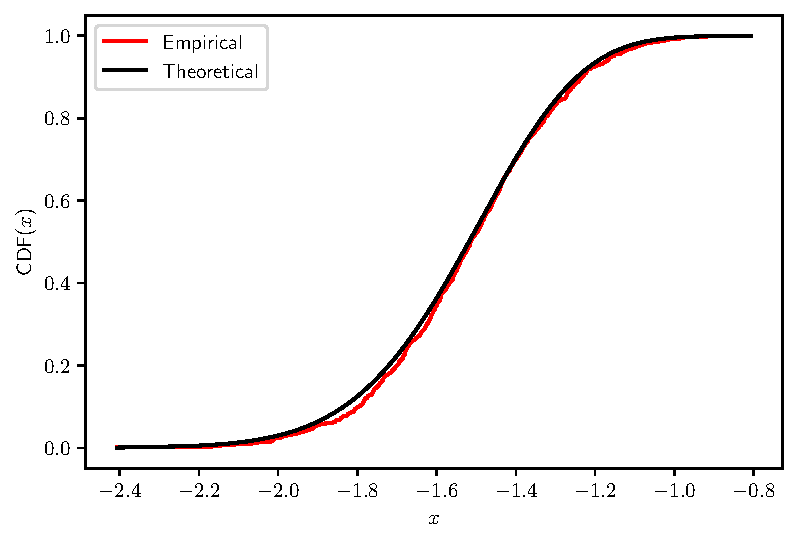
\includegraphics[scale=0.5]{../figs/order.pdf}
    \caption{Comparison between ECDF and theoretic distribution.}
    \label{fig:ex7}
  \end{figure}
\end{proof}

\subsection*{Exercise 8}
Suppose $X$ is an exponentially random variable of parameter
$\beta$. Calculate:

$$P(|X-\mu|>k \sigma)$$

for $k>1$.

\begin{proof}
  Recall Chebyshev's inequality: let $Y$ be a random variable and let
  $\E{Y}=\mu$ and $\V{Y}=\sigma^2$, then

\[
  P(|Y-\mu|\geq t)\leq\dfrac{\sigma^2}{t^2}.
\]

Let
\begin{align*}
  P(|X-\mu|>k \sigma) &=P(-k \sigma>X-\mu>k \sigma) \\
                      &=P(-k \sigma+\mu>X>k \sigma+\mu) \\
                      &=P(X<\mu-k \sigma)+P(X>k \sigma+\mu) \\
                      &=P\left(X<\frac{1-k}{\beta}\right)+1-P\left(X<\frac{k+1}{\beta}\right) \quad \text { but } 1-k<0\\
                      &=1-\left(1-e^{-\frac{k+1}{\beta^{2}}}\right) \\
                      &=P(|X-\mu|>k \sigma)\\
                      &\leq \frac{\sigma^{2}}{(k \sigma)^{2}} \\
                      &\leq \frac{1}{k^{2}}
\end{align*}

Clearly $e^{-\frac{k+2}{\beta^{2}}}$ is always lesser than $1$ and
because $k>1$ then $\frac{1}{k^{2}}$ is also lesser than one. Thus,
$P(|X-\mu|>k \sigma)$ is bounded by Chebyshev's inequality.
\end{proof}


\subsection*{Exercise 9}
Prove that if $X\sim \mathrm{Poisson}(\lambda)$, then
\[
  P(X\geq 2\lambda)\leq \dfrac{1}{\lambda}.
\]
\begin{proof}
  Let $X\sim \mathrm{Poisson}(\lambda)$. Recall Chebyshev's
  inequality: let $Y$ be a random variable and let $\E{Y}=\mu$ and
  $\V{Y}=\sigma^2$, then
\[
  P(|Y-\mu|\geq t)\leq\dfrac{\sigma^2}{t^2}.
\]
Clearly, $\E{X}=\V{X}=\lambda$. If we set $t=\lambda$, then
\[
\begin{split}
  P(|X-\lambda|\geq\lambda)&\leq\dfrac{1}{\lambda}\\
  P\left[(X-\lambda\geq\lambda)\cup(X-\lambda\leq-\lambda)\right]&\leq\dfrac{1}{\lambda}\\
  P\left[(X\geq2\lambda)\cup(X\leq0)\right]&\leq\dfrac{1}{\lambda}\\
  P(X\geq2\lambda)+P(X\leq0)&\leq\dfrac{1}{\lambda}\\
  P(X\geq 2\lambda)&\leq \dfrac{1}{\lambda}
\end{split}
\]
\end{proof}

\subsection*{Exercise 10}
\begin{definition}
  The sequence $\{X_n\}$ of random variables is said to converge in
  probability to $X$ if
\[
\forall\epsilon>0, \ \lim_{n\rightarrow\infty}P\left(|X_n-X|>\epsilon\right)=0
\]
\end{definition}

\begin{definition}
  The sequence $\{X_n\}$ of random variables is said to converge in
  mean-square to $X$ if
\[
  \lim_{n\rightarrow\infty}\E{(X_n-X)^2}=0
\]
\end{definition}
\begin{theorem}
  The convergence in mean-square implies convergence in probability.
\end{theorem}

\begin{proof}
  Let $\{X_n\}$ be a sequence of random variables that converges in
  mean-square to $X$. Recall Markov's inequality: Let $Y$ be a
  non-negative random variable and suppose $\E{Y}$ exists. Then for
  any $t>0$,
\[
  P(Y>t) \leq \dfrac{\E{Y}}{t}.
\]
Take $Y=|X_n-X|$ and $t=\epsilon$, then
\[
\begin{split}
  P(|X_n-X|>\epsilon) &= P\left[(X_n-X)^2>\epsilon^2\right]\\
  & \leq \dfrac{\E{(X_n-X)^2}}{\epsilon^2}
\end{split}
\]
Since $\{X_n\}$ converges in mean-square to $X$, $\E{(X_n-X)^2}\rightarrow0$ as $n\rightarrow\infty$, which directly
implies that $P(|X_n-X|>\epsilon)\rightarrow0$ as
$n\rightarrow\infty$.
\end{proof}


\subsection*{Exercise 11}
Show that the ECDF converges in probability to the theoretical
continuous distribution function.
\begin{proof}
  Let $X_i$, for $i=1,\ldots,n$, be a independent data sample. Then,
  the empirical distribution function is defined as
  \begin{equation*}
    \hat{F}_n(x) = \frac{1}{n} \sum_{i=1}^nI(X_i \le x)
  \end{equation*}
  where
  \begin{equation*}
    I(X_i \le x) =
    \begin{cases}
      1 &\text{if } X_i \le x \\
      0 &\text{otherwise}
    \end{cases}
  \end{equation*}

  Hence, to see that it converges in probability lets see if the MSE
  tends to 0 when the number of samples is bigger. Let's calculate the
  expectancy of the estimator.
  \begin{align*}
    \E{\hat{F}_n(x)} &= \E{\frac{1}{n}\sum_{i=1}^nI(X_i \le x)} \\
                     &=\frac{1}{n}\sum_{i=1}^n \E{I(X_i \le x)} \\
                     &= \frac{1}{n} \sum_{i=1}^n \P{X_i \le x} \\
                     &= \frac{1}{n} \sum_{i=1}^nF(x) \\
                     &= F(x)
  \end{align*}
  In this manner, it is a non-biased estimator for the theoretical
  distribution. Hence, the MSE is calculated by the variance. Then:
  \begin{align*}
    \mathrm{MSE} &= \V{\hat{F}_n(x)} + \mathrm{Bias}\left(\hat{F}_n(x), F(x)\right)\\
                 &= \V{\frac{1}{n} \sum_{i=1}^n I(X_i \le x)} \\
                 &= \frac{1}{n^2} \sum_{i=1}^n \V{I(X_i \le x)} \\
                 &= \frac{1}{n^2} \sum_{i=1}^n \left[\P{X_i \le x}(1 - \P{X_i \le x})\right] \\
                 &= \frac{1}{n^2} \sum_{i=1}^n \left[F(x)(1 - F(x))\right] \\
                 &= \frac{F(x)(1 - F(x))}{n}
  \end{align*}
  Hence, when $n \rightarrow \infty$ the MSE tends to 0. Therefore,
  \begin{equation*}
    \hat{F}_n(x) \xrightarrow[]{P} F(x)
  \end{equation*}
\end{proof}

\subsection*{Exercise 12}
Consider the daily temperatures of the hottest year in
average. Calculate a confidence interval for the maximum
temperature. Calculate the bias of $T_{[n]}$ and the variance.

\begin{proof}
  To calculate the interval for the maximum temperature, we applied
  the normal bootstrap method. The normal bootstrap method consists
  of, in a sample $X_1, \ldots, X_n$ and a confidence of $1 - \alpha$:
  \begin{enumerate}
  \item First, extract $k$ samples of the size $n$ with repetition and
    calculate the desired statistic to find it's confidence
    intervals.  Let $S_i$ be the sample of each statistic calculated.
  \item Calculate:
    \begin{equation*}
      v_{\text{boot}} = \frac{1}{k} \sum_{i=1}^k\left(S_i - \frac{1}{n}
        \sum_{i=1}^k S_i\right)^2
     \end{equation*}
   \item Then, the interval of confidence for the statistic is, with
     $S$ the statistic calculated in the original sample:
     \begin{equation*}
       (S - z_{\alpha/2} \sqrt{v_{\text{boot}}} , S + z_{\alpha/2} \sqrt{v_{\text{boot}}})
     \end{equation*}
     where $z_{\alpha/2}$ is the $1 - \alpha / 2$ quantile of a
     standard normal distribution.
   \end{enumerate}
   The result for the maximum temperatures interval is, with
   $\alpha=0.05$ and $k = 1000$:
   \begin{equation*}
     T_{[n]} \in (18.486, 18.714)
   \end{equation*}

   On the other hand, to calculate the variance and bias the Jackknife
   method was used. The Jackknife method consists is explained in the
   following exercise. Hence, we find that the bias and the variance
   and we obtain:
   \begin{align*}
     b_{\text{jack}} &= -0.10 \\
     v_{\text{jack}} &= 7.49 \cdot 10^{-8}
   \end{align*}
 \end{proof}

 \subsection*{Exercise 13}
 In this section, a sample of a uniform distribution in the interval
 [0,1] is generated. Then a bootstrap method to calculate the variance
 and a Jackknife method to calculate the bias of this sample are
 implemented.

The bootstrap and the jackknife are non-parametric methods for
computing standard errors and confidence intervals \cite{rodgers1999bootstrap}. A short review of the methodology will be presented, based on \cite{wasserman2006}.

\subsubsection*{The Jackknife}

Jackknife is a simple method for approximating the bias and variance
of an estimator. Let $T_{n}=T\left(X_{1}, \ldots, X_{n}\right)$ be an
estimator of some quantity $\theta$ and let
$\operatorname{bias}\left(T_{n}\right)=\mathbb{E}\left(T_{n}\right)-\theta$
denote the bias. Let $T_{(-i)}$ denote the statistic with the
$i^{\text {th }}$ observation removed. The jackknife bias estimate is
defined by
\[
  b_{\mathrm{jack}}=(n-1)\left(\bar{T}_{n}-T_{n}\right)
\]

where $\bar{T}_{n}=n^{-1} \sum_{i} T_{(-i)}$. The bias-corrected
estimator is $T_{\mathrm{jack}}=T_{n}-b_{\mathrm{jack}}$

\subsubsection*{The Bootstrap}

Bootstrap is a method for estimating the variance and the distribution
of a statistic $T_{n}=g\left(X_{1}, \ldots, X_{n}\right) .$

Let $\mathbb{V}_{F}\left(T_{n}\right)$ denote the variance of
$T_{n} .$ We have added the subscript $F$ to emphasize that the
variance is a function of $F$. If we knew $F$ we could, at least in
principle, compute the variance. For example, if
$T_{n}=n^{-1} \sum_{i=1}^{n} X_{i}$ then
\[
  \mathbb{V}_{F}\left(T_{n}\right)=\frac{\sigma^{2}}{n}=\frac{\int
    x^{2} d F(x)-\left(\int x d F(x)\right)^{2}}{n}
\]
which is clearly a function of $F$.

With the bootstrap, we estimate $\mathbb{V}_{F}\left(T_{n}\right)$
with $\mathbb{V}_{\widehat{F}_{n}}\left(T_{n}\right)$. In other words,
we use a plug-in estimator of the variance. since,
$\mathbb{V}_{\widehat{F}_{n}}\left(T_{n}\right)$ may be difficult to
compute, we approximate it with a simulation estimate denoted by
$v_{\text {boot }}$
\\

Its important to know that The jackknife is a linear approximation of
the bootstrap.
\\

In the simulation, the Variance Bootstrap obtained from the uniform
sample of the Order statistic is
$v_{\text {boot }} = 3.5815$x$10^{-8}$, this indicates that almost all
of the Order data values are nearly identical. Moreover, the
theoretical bias and the Jackknife bias generated similar results,
$b_{\mathrm{jack}}$ = $-1.6166$x$10^{-5}$ and
$b_{\mathrm{theoretical}}$ = $-9.9990$x$10^{-5}$, which shows that the
bias of the estimator is unbiased, hence the sampling distribution has
a mean that is equal to the parameter being estimated.


It should be noted that the jackknife method is less computationally
expensive, but the bootstrap has some statistical advantages, such as
its simplicity to derive estimates of standard errors and confidence
intervals for complex estimators of complex parameters of the
distribution.


\subsection*{Exercise 14}
Show the differences between the parametric and non-parametric
bootstrap. Investigate robust versions of the bootstrap method and
show examples about their performance.

\begin{proof}
  Following the ideas from \cite{wasserman2006} and
  \cite{kulperger2018}, Bootstrap is performed over a sample
  $X_1,...,X_n$. In the case of the nonparametric Bootstrap, we
  generate new samples (resampling) based on the ECDF $\hat{F}_n$ of
  the sample; the generation of samples from the ECDF is equivalent to
  draw samples $X_1^j,...,X_n^j$ from the original data \textbf{with
    replacement} for $j=1,...,N$, where $N$ is the number of Bootstrap
  resamples. On the other hand, the parametric Bootstrap takes into
  consideration that the data comes from an specific distribution
  $F_\theta$ that, clearly, depends on an unknown parameter $\theta$;
  instead of drawing from $\hat{F}_n$, we draw from
  $F_{\hat{\theta}}$, where $\hat{\theta}$ is an estimator of $\theta$
  based on the sample. This method is just as accurates as the
  nonparametric, but under certain scenarios could not behave
  properly. An excellent example of the parametric and nonparametric
  Bootstrap is presented in point 11 of page 40 from
  \cite{wasserman2006}.

\end{proof}

\subsection*{Exercise 15}
The data used in this section is bivariate, taking the temperature
from the years that are, in average, the coldest and hottest. Let
$\boldsymbol{\mathrm{Y}}\in\mathbb{R}^{n\times2}$ be the set of
bivariate samples of size $n$ (data matrix). In our case, $n=365$
days.


The usual cutout of outliers in elliptical data (e.g. bivariate
normally distributed data) is made using the $\chi^2$
distribution. However, the bivariate data obtained from the
temperatures is not guaranteed to follow such elliptical
behavior. Therefore, the usual cutout will be done with the same
methodology as the robust variations. The methods for estimating the
covariance matrix will be first presented, then the methodology to
remove outliers will be described and finally the results will be
presented.

\subsubsection*{Usual Estimation}
\begin{definition}
  Let $\boldsymbol{\mathrm{x}}$ be an multivariate observation from a
  set of observations with mean vector $\boldsymbol{\mu}$ and
  covariance matrix $\Sigma$. The Mahalanobis distance of the
  observation $\boldsymbol{\mathrm{x}}$ is
\begin{equation}\label{eq:mahal}
  d^2(\boldsymbol{\mathrm{x}}) = (\boldsymbol{\mathrm{x}} - \boldsymbol{\mu})^T\Sigma^{-1}(\boldsymbol{\mathrm{x}} - \boldsymbol{\mu}).
\end{equation}

\end{definition}

Clearly, the usual cutout is performed using the natural estimation of
the Mahalanobis distance, using the standard unbiased estimators of
the mean vector and covariance matrix from the data matrix
$\boldsymbol{\mathrm{Y}}$, presented respectively in Equation
(\ref{eq:nat_est}), where $\boldsymbol{\mathrm{y}}_i$ is the $i$-th
row of the data matrix $\boldsymbol{\mathrm{Y}}$.

\begin{equation}\label{eq:nat_est}
  \hat{\boldsymbol\mu}=\bar{\boldsymbol{\mathrm{y}}}=\left[\dfrac{1}{n}\sum_{i=1}^{n}\boldsymbol{\mathrm{y}}_i\right]^T,\quad \hat{\Sigma}=S=\dfrac{1}{n-1}\sum_{i=1}^{n} (\boldsymbol{\mathrm{y}}_i^T-\bar{\boldsymbol{\mathrm{y}}})(\boldsymbol{\mathrm{y}}_i^T-\bar{\boldsymbol{\mathrm{y}}})^T
\end{equation}

\subsubsection*{Comedian Estimation}

The first robust calculation of the Mahalanobis distance is based on a
robust estimation of the covariance matrix following the ideas from
\cite{falk1997mad}, using the following definition.
\begin{definition}
  Let $X$ and $Y$ be random variables. The comedian between $X$ and
  $Y$ is defined as
\[
  \mathrm{Com}(X,Y)=\mathrm{Med}\left[(X-\mathrm{Med}(X))(Y-\mathrm{Med}(Y))\right]
\]
\end{definition}
The covariance matrix is then estimated by applying the comedian to
each entry. Then the Mahalanobis distance formula is applied using
this matrix and the median vector instead of the mean.

\subsubsection*{Kendall Estimation}
This method uses the Kendall rank correlation coefficient, usually
known as Kendall's $\tau$ coefficient, originally proposed in
\cite{kendall1938new}. Each entry of the covariance matrix is
estimated using
\[
  \mathrm{Cov}(X,Y)=\rho_kS_XS_Y,
\]
where $\rho_k$ is Kendall's $\tau$ coefficient, and $S_X$ and $S_Y$
are the respective standard deviations.

\subsubsection*{Spearman Estimation}
This estimation was performed similarly to Kendall's. The covariance
matrix is estimated using
\[
  \mathrm{Cov}(X,Y)=\rho_sS_XS_Y,
\]
where $\rho_s$ is Spearman's correlation coefficient (see
\cite{ce1904general}), and $S_X$ and $S_Y$ are the respective standard
deviations.

\subsubsection*{Cutout Procedure}
As previously mentioned, the cutout method is performed with the same
procedure for all the covariance matrix estimations. The procedure is
presented as follows:
\begin{enumerate}
\item Estimate the covariance matrix accordingly to the estimation
  method.
  \item Apply equation (\ref{eq:mahal}) to each bivariate data, with
    the estimation of the covariance matrix from step 1 and the
    corresponding estimated mean vector.
  \item Fit a continuous distribution to the vector of squared
    distances: take the available continuous distributions from
    Python's package SciPy, fit each distribution to the squared
    distances and apply a Kolmogorov-Smirnov goodness-of-fit test in
    order to rank the fitted distributions. Keep the best fit.
  \item Calculate the $\alpha/2$ and $1-\alpha/2$ quantiles of the fitted distibution.
  \item Mark the outliers as the data points that are beyond the
    quantiles obtained on step 4.
\end{enumerate}


\subsubsection*{Results}
In Figure \ref{fig:scatter} shows the scatter plot of the bivariate
data used in this section.

\begin{figure}[H]
  \centering 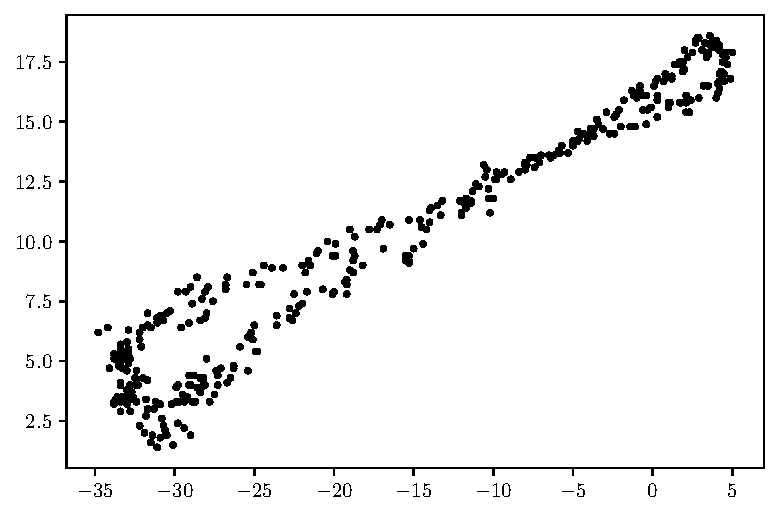
\includegraphics[scale=.5]{../figs/scatter.pdf}
  \caption{Scatter plot of bivariate data.}
  \label{fig:scatter}
\end{figure}

The first cut method was done with the usual estimation of the
covariance matrix. In Figure \ref{fig:nrob_cut_nnoise}, the results
for this procedure are presented. The best-fit was a Mielke's
Beta-Kappa distribution, whose probability density function(p.d.f.) is
\[
f(t)=\dfrac{kt^{k-1}}{(1+t^s)^{1+\frac{k}{s}}},\quad t>0
\]
with parameters $k=0.96$, $s=3.85$, loc=0.01 and scale=3.37, and it
was not rejected with a p-value of $0.34$.

\begin{figure}[H]
  \centering
  \begin{subfigure}[t]{0.475\textwidth}
    \centering
    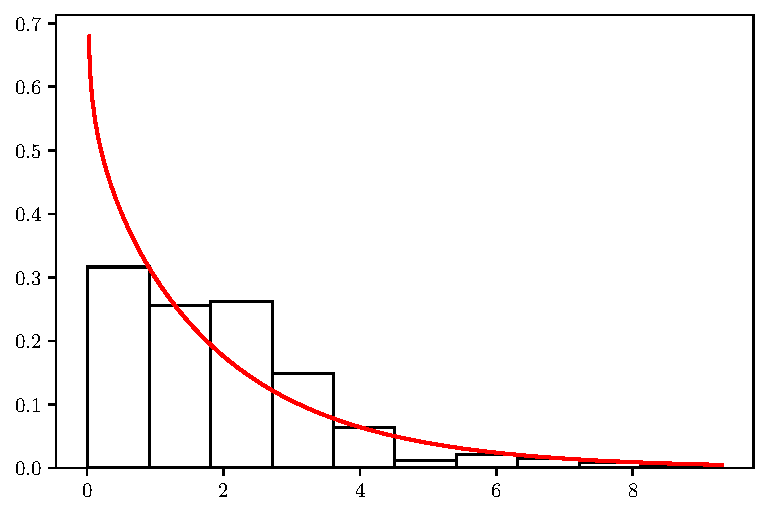
\includegraphics[scale=0.45]{../figs/non_robust_hist_no-noise.pdf}
    \caption{Fitted distribution.}
  \end{subfigure}
  \begin{subfigure}[t]{0.475\textwidth}
    \centering
    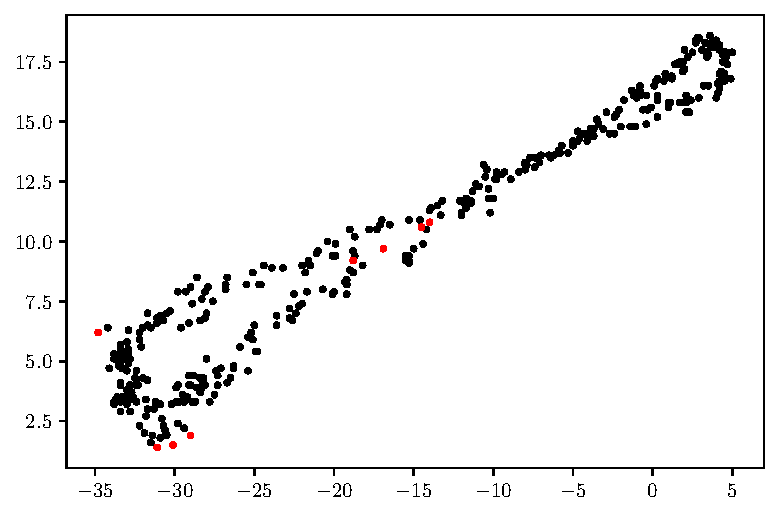
\includegraphics[scale=0.45]{../figs/non_robust_scatter_no-noise.pdf}
    \caption{Outliers cutout.}
    \end{subfigure}
  \caption{Results using the usual estimation.}
  \label{fig:nrob_cut_nnoise}
\end{figure}

On the other hand, the first robust approach is usig the Comedian
procedure above described, where each entry is estimated using the
comedian and the mean vector is replaced with the median vector. The
results are shown in Figure \ref{fig:comedian_cut_nnoise}. The
best-fit was an inverse gaussian distribution, whose density is given
by
\[
  f(t)=\dfrac{1}{\sqrt{2\pi t^3}}e^{-\frac{(t-\mu)^2}{2t\mu^2}}, \quad
  t>0
\]
with parameters $\mu=1.11$, loc=-254.79 and scale=2667.77, and it not
rejected with a p-value of $0.28$.
\begin{figure}[H]
  \centering
  \begin{subfigure}[t]{0.475\textwidth}
    \centering
    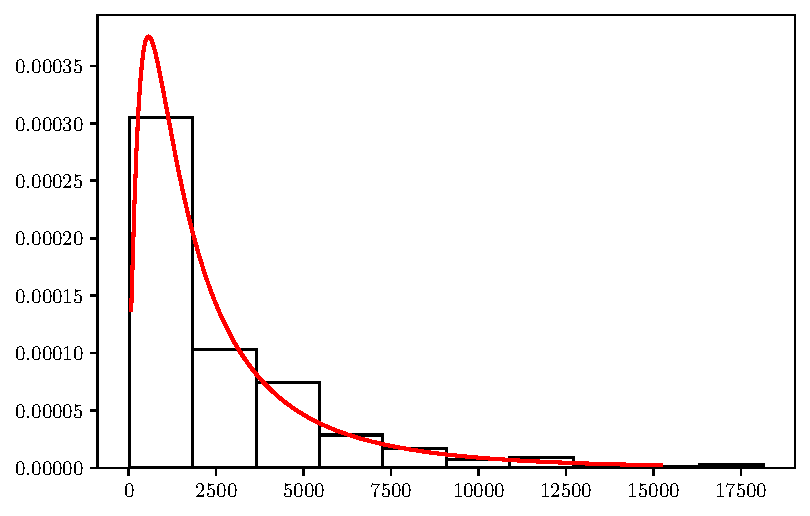
\includegraphics[scale=0.45]{../figs/comedian_hist_no-noise.pdf}
      \caption{Fitted distribution.}
    \end{subfigure}
  \begin{subfigure}[t]{0.475\textwidth}
    \centering
    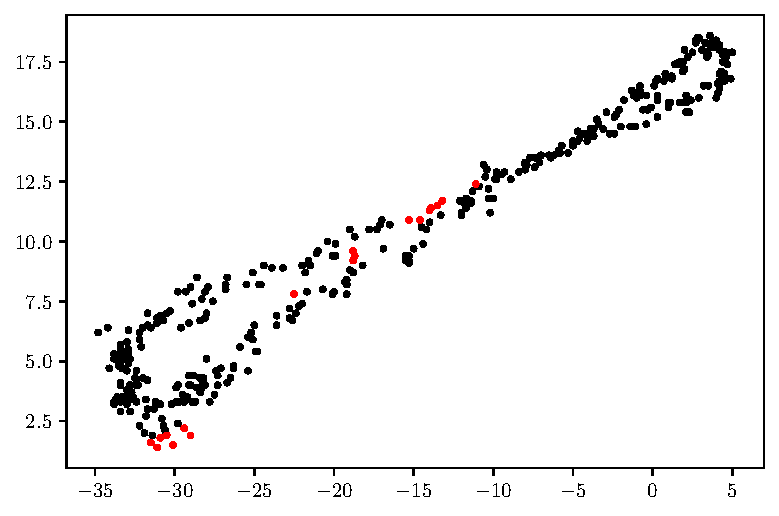
\includegraphics[scale=0.45]{../figs/comedian_scatter_no-noise.pdf}
      \caption{Outliers cutout.}
    \end{subfigure}
  \caption{Results using the comedian estimation.}
  \label{fig:comedian_cut_nnoise}
\end{figure}


Furthermore, the same procedure was carried out using the covariance
matrix estimation based on Kendall's $\tau$ correlation
coefficient. Figure \ref{fig:kendall_cut_nnoise} shows the obtained
results for the bivariate data.  The best-fit was a folded normal
distribution, whose p.d.f is given by
\[
  f(t)=\sqrt{\dfrac{2}{\pi}}\cosh{(ct)}e^{-\frac{(t^2+c^2)}{2}},\quad
  t>0
\]
with parameters $\mu=1.01$, loc=0 and scale=2.19, and it was not
rejected with a p-value of 0.45.
\begin{figure}[H]
  \centering
  \begin{subfigure}[t]{0.475\textwidth}
    \centering
    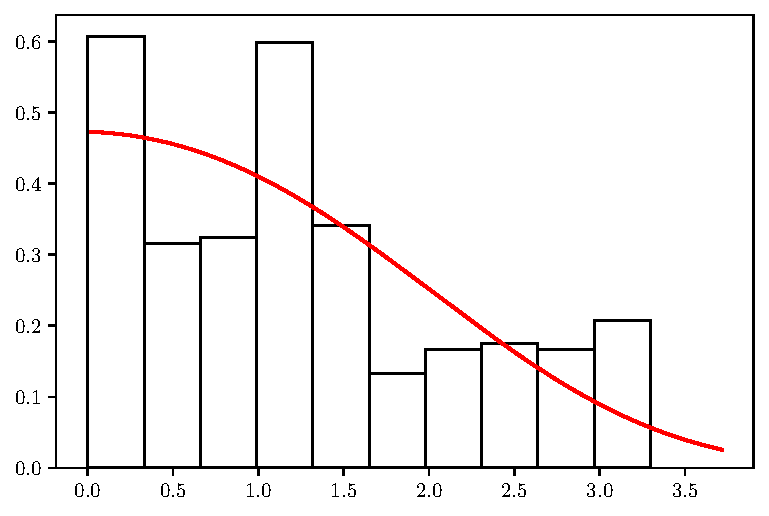
\includegraphics[scale=0.45]{../figs/kendall_hist_no-noise.pdf}
    \caption{Fitted distribution.}
  \end{subfigure}
  \begin{subfigure}[t]{0.475\textwidth}
    \centering
    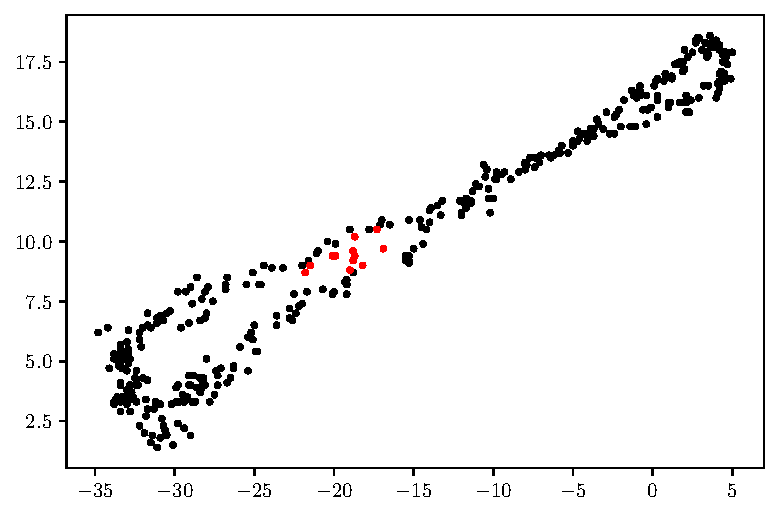
\includegraphics[scale=0.45]{../figs/kendall_scatter_no-noise.pdf}
    \caption{Outliers cutout.}
    \end{subfigure}
  \caption{Results using Kendall estimation.}
  \label{fig:kendall_cut_nnoise}
\end{figure}

Finally, the last robust estimation of the covariance matrix was
constructed using Spearman's correlation coefficient and the outlier
detection results are presented in Figure
\ref{fig:spearman_cut_nnoise}. The best-fit was a Gompertz
distribution, whose p.d.f. is given by
\[
  f(t)=ce^{t}e^{-ce^{t}-1},\quad t>0
\]
with parameters $c=1.04$, loc=0 and scale=2.19, and it was not
rejected with a p-value of 0.31.

\begin{figure}[H]
  \centering
  \begin{subfigure}[t]{0.475\textwidth}
    \centering
    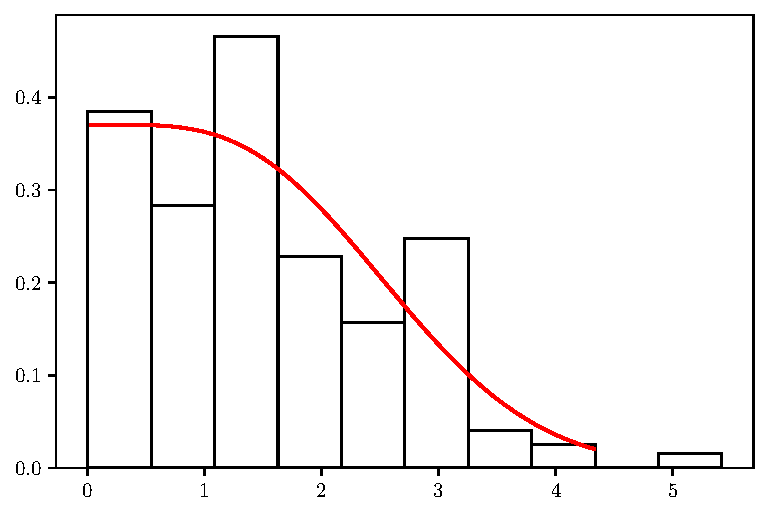
\includegraphics[scale=0.45]{../figs/spearman_hist_no-noise.pdf}
    \caption{Fitted distribution.}
    \end{subfigure}
  \begin{subfigure}[t]{0.475\textwidth}
    \centering
    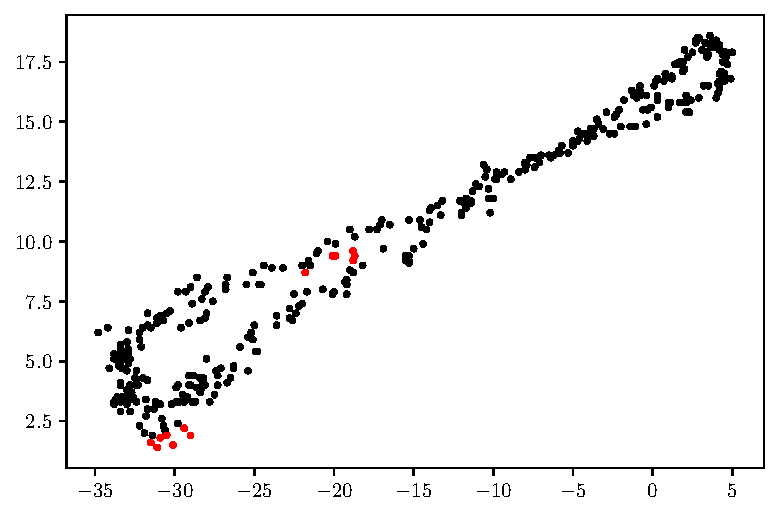
\includegraphics[scale=0.45]{../figs/spearman_scatter_no-noise.pdf}
    \caption{Outliers cutout.}
    \end{subfigure}
  \caption{Results using Spearman estimation.}
  \label{fig:spearman_cut_nnoise}
\end{figure}

In the following results, the same procedures of outlier cutout is
presented, but taking a "damaged" sample. This new sample takes 30
random bivariate observations and adds normally distributed
observations, with mean 10 and standard deviation of 0.5. The results
for the usual, the comedian, the Kendall and the Spearman cutouts are
presented, respectively, in Figures \ref{fig:nrob_cut_wnoise},
\ref{fig:comedian_cut_wnoise}, \ref{fig:kendall_cut_wnoise} and
\ref{fig:spearman_cut_wnoise}. It is important to highlight that the
fitting was done assuming the same distributions from the previous
procedures.

\begin{figure}[H]
  \centering
  \begin{subfigure}[t]{0.475\textwidth}
    \centering
    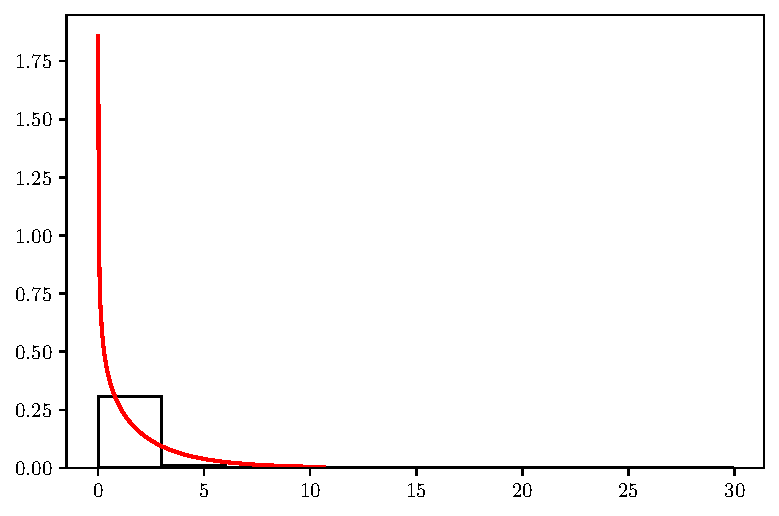
\includegraphics[scale=0.45]{../figs/non_robust_hist_with-noise.pdf}
    \caption{Fitted distribution.}
  \end{subfigure}
  \begin{subfigure}[t]{0.475\textwidth}
    \centering
    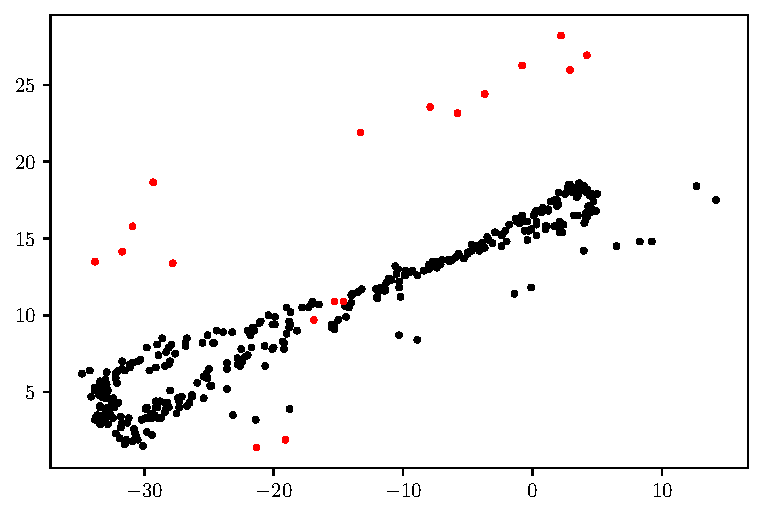
\includegraphics[scale=0.45]{../figs/non_robust_scatter_with-noise.pdf}
    \caption{Outliers cutout.}
  \end{subfigure}
  \caption{Results using the usual estimation on contaminated data.}
  \label{fig:nrob_cut_wnoise}
\end{figure}
\begin{figure}[H]
  \centering
  \begin{subfigure}[t]{0.475\textwidth}
    \centering
    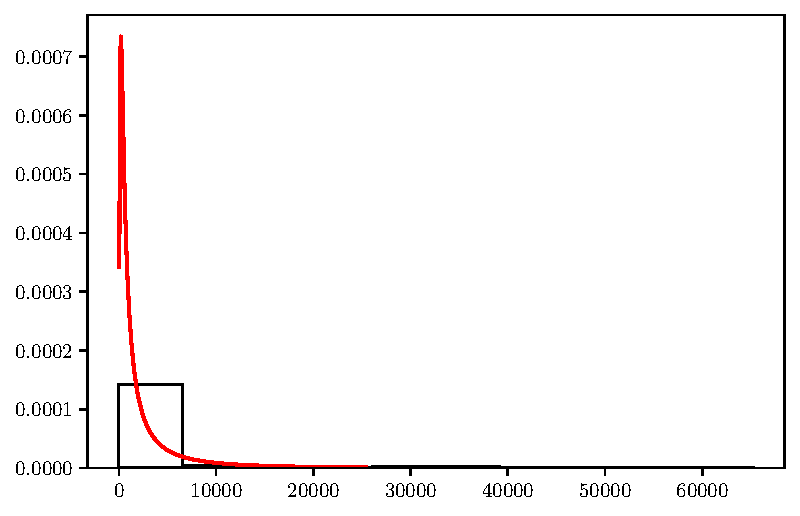
\includegraphics[scale=0.45]{../figs/comedian_hist_with-noise.pdf}
    \caption{Fitted distribution.}
  \end{subfigure}
  \begin{subfigure}[t]{0.475\textwidth}
    \centering
    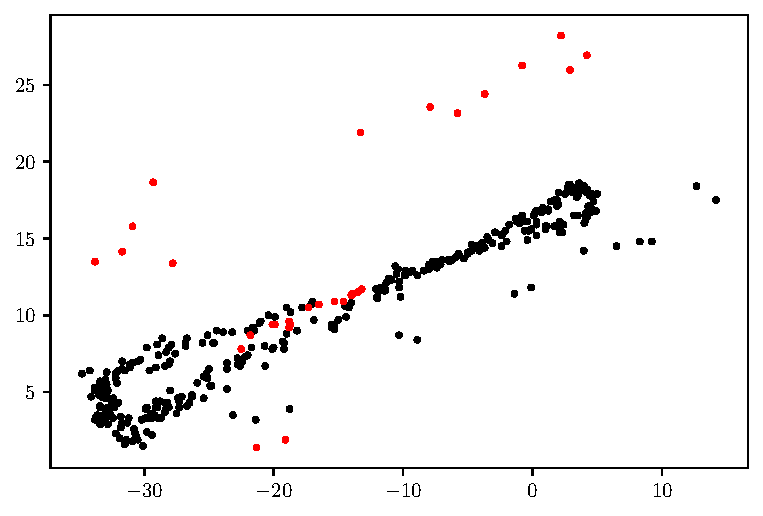
\includegraphics[scale=0.45]{../figs/comedian_scatter_with-noise.pdf}
    \caption{Outliers cutout.}
  \end{subfigure}
  \caption{Results using the comedian estimation on contaminated
    data.}
  \label{fig:comedian_cut_wnoise}
\end{figure}
\begin{figure}[H]
  \centering
  \begin{subfigure}[t]{0.475\textwidth}
    \centering
    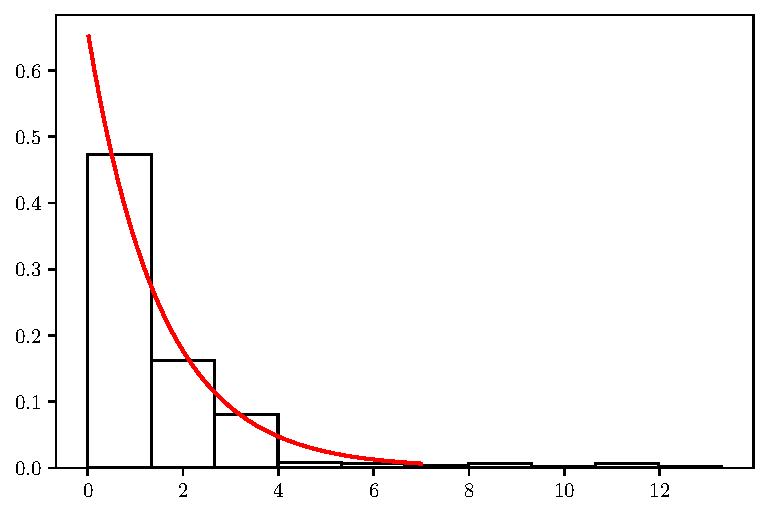
\includegraphics[scale=0.45]{../figs/kendall_hist_with-noise.pdf}
    \caption{Fitted distribution.}
  \end{subfigure}
  \begin{subfigure}[t]{0.475\textwidth}
    \centering
    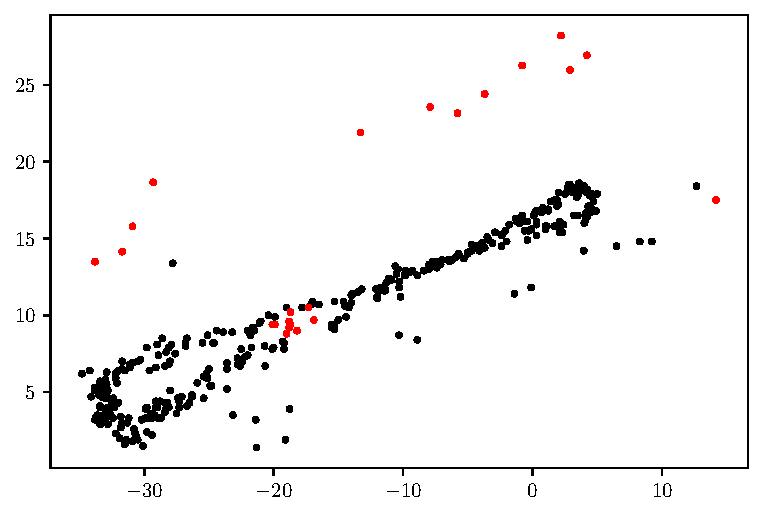
\includegraphics[scale=0.45]{../figs/kendall_scatter_with-noise.pdf}
    \caption{Outliers cutout.}
  \end{subfigure}
  \caption{Results using Kendall estimation on contaminated data.}
  \label{fig:kendall_cut_wnoise}
\end{figure}
\begin{figure}[H]
  \centering
  \begin{subfigure}[t]{0.475\textwidth}
    \centering
    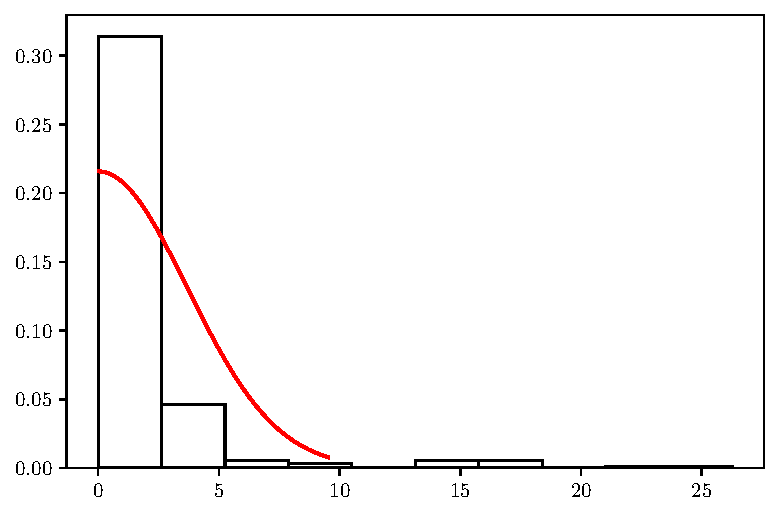
\includegraphics[scale=0.45]{../figs/spearman_hist_with-noise.pdf}
    \caption{Fitted distribution.}
  \end{subfigure}
  \begin{subfigure}[t]{0.475\textwidth}
    \centering
    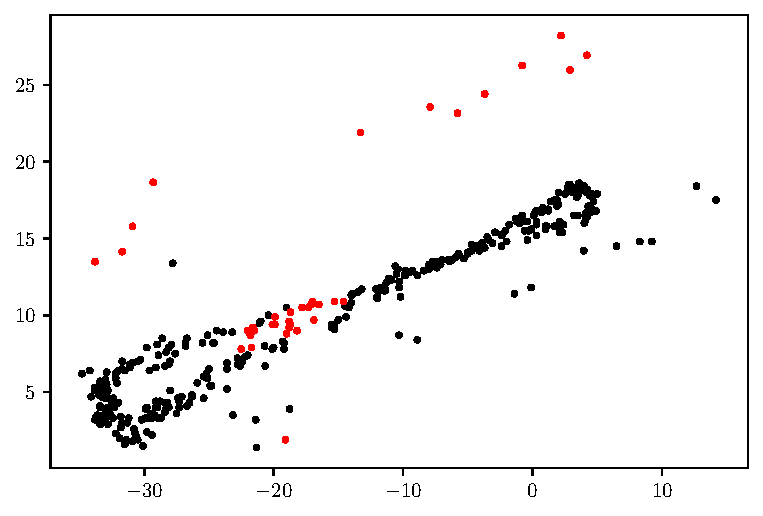
\includegraphics[scale=0.45]{../figs/spearman_scatter_with-noise.pdf}
    \caption{Outliers cutout.}
  \end{subfigure}
  \caption{Results using Spearman estimation on contaminated data.}
  \label{fig:spearman_cut_wnoise}
\end{figure}


\section{Book Exercises}
All exercises in this section are extracted from \parencite{wasserman2006}.

\subsection{Page 10, Exercise 2}
Let $X_{1}, \ldots, X_{n} \sim$ Bernoulli $(p) .$ A pointwise
asymptotic $1-\alpha$ confidence interval for $p$ is
\[
  \widehat{p}_{n} \pm z_{\alpha / 2}
  \sqrt{\frac{\widehat{p}_{n}\left(1-\widehat{p}_{n}\right)}{n}}
\]
where $\widehat{p}_{n}=n^{-1} \sum_{i=1}^{n} X_{i} .$ It follows from
Hoeffding's inequality that a finite sample confidence interval is
\[
  \widehat{p}_{n} \pm \sqrt{\frac{1}{2 n} \log
    \left(\frac{2}{\alpha}\right)}
\]

In Figure \ref{fig:bands} is presented the coverage and length of the
pointwise asymptotic $1-\alpha$ confidence interval and the finite
sample confidence interval (Hoeffding) to estimate the $p$ parameter
of a Bernoulli distribution. To simulated this scenario a Bernoulli
distribution was generate with parameters $p$ = 0.2 and $\alpha$ =
.05.

\begin{figure}[H]
    \centering
    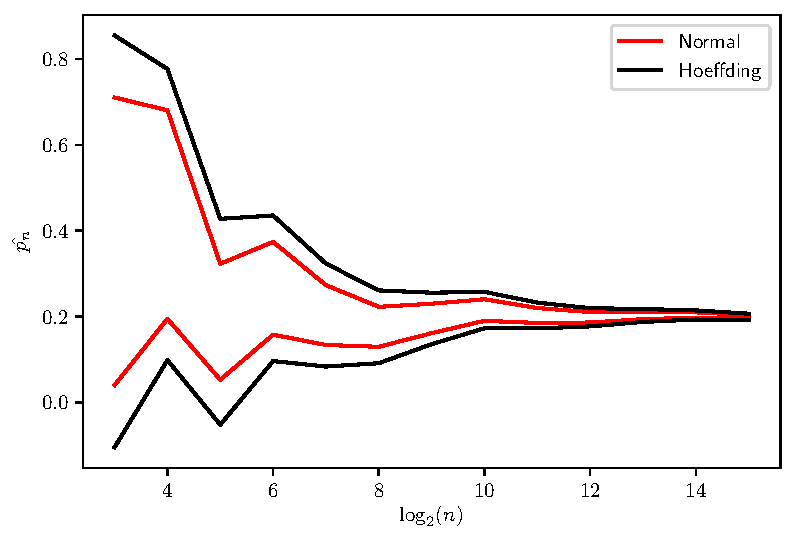
\includegraphics[scale=.5]{../figs/bernoulli_bands.pdf}
    \caption{Confidence bands for the value of $p$.}
    \label{fig:bands}
\end{figure}

The result shows that an large sample must be generated so that the
pointwise interval has accurate coverage of the $p$, it can also be
seen that both intervals have similar length when reaching an accurate
coverage, being Hoeffding the interval with the highest coverage due
to a very slight difference.

Note that the sample sizes shown on the graph are in powers.

\subsection*{Page 24, Exercise 3}
This exercise uses a sample of 100 observations that are normally
(standard) distributed. It is required to compute a 95\% confidence
band for the CDF $F$ and how many times this band covers the true CDF
of the data, by repeating the process 1000 times. For this procedure
we use the bands derived from Dvoretzky–Kiefer–Wolfowitz inequality
\cite{wasserman2006}. In Figures \ref{subfig:worst_band_normal} and
\ref{subfig:best_band_normal} we present the worst and best band
obtained over the experiments, respectively. The experiments yield
that only 8 out of the 1000 bands simulated contain the true CDF of
the standard normal random variable.

\begin{figure}[H]
  \centering
  \begin{subfigure}[t]{0.475\textwidth}
      \centering
      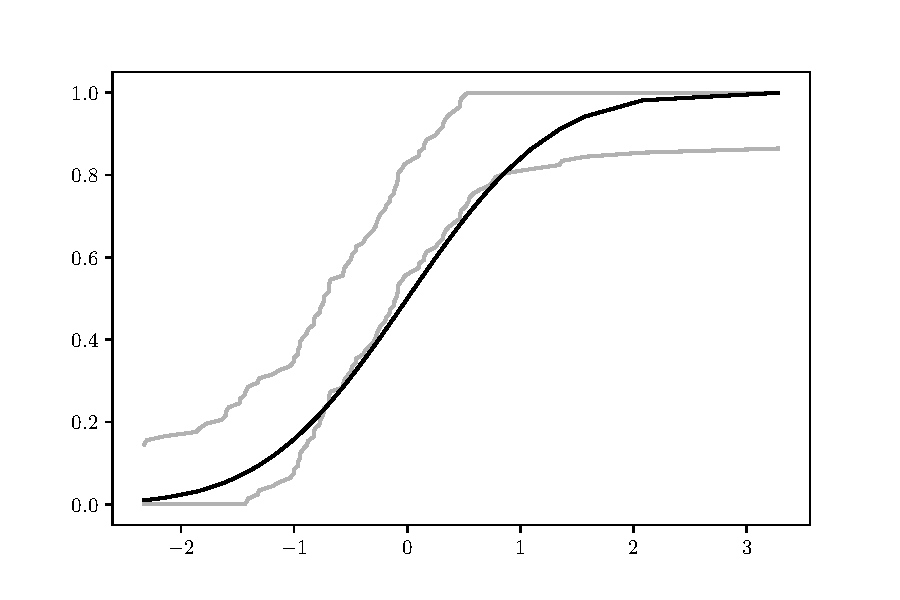
\includegraphics[scale=0.45]{../figs/min_normal_bands.pdf}
      \caption{Worst enclosing band.}
      \label{subfig:worst_band_normal}
  \end{subfigure}
  \begin{subfigure}[t]{0.475\textwidth}
      \centering
      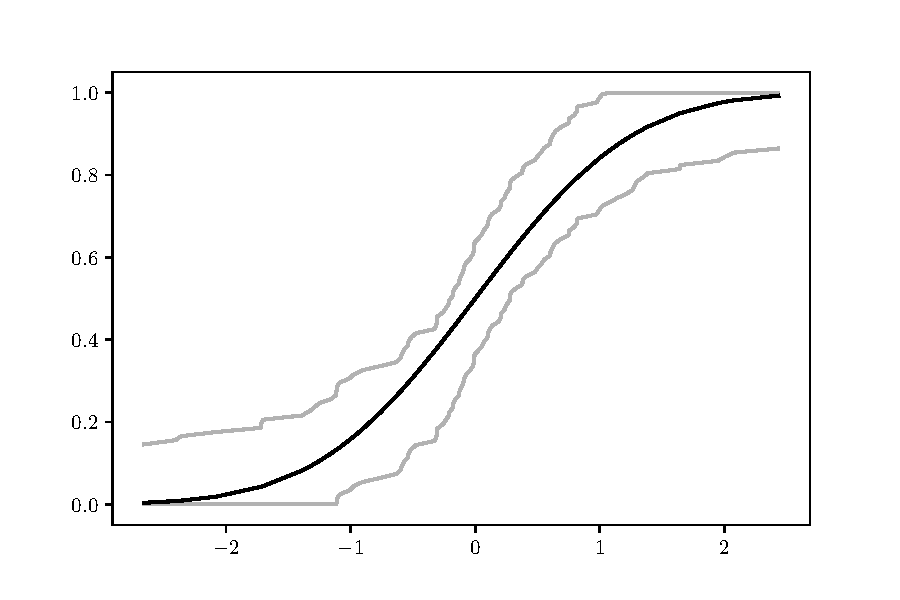
\includegraphics[scale=0.45]{../figs/max_normal_bands.pdf}
      \caption{Best enclosing band.}
      \label{subfig:best_band_normal}
  \end{subfigure}
  \caption{Confidence bands for $F$ of normal data.}
  \label{fig:bands_normal}
\end{figure}

Additionally, the experiment was repeated with a Cauchy distribution
with p.d.f. given by
\[
  f(t)=\dfrac{1}{\pi(1+t^2)},\quad\forall t\in\mathbb{R}.
\]
The obtained result are presented in Figure \ref{fig:bands_cauchy}, as
well with the worst and best enclosing bands.
\begin{figure}[H]
  \centering
  \begin{subfigure}[t]{0.475\textwidth}
      \centering
      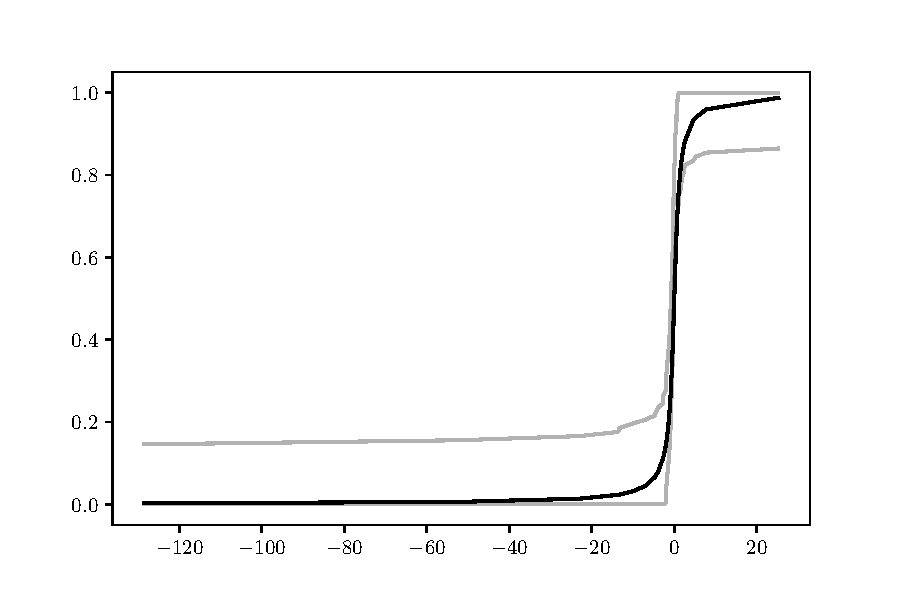
\includegraphics[scale=0.45]{../figs/min_cauchy_bands.pdf}
      \caption{Worst enclosing band.}
      \label{subfig:worst_band_cauchy}
  \end{subfigure}
  \begin{subfigure}[t]{0.475\textwidth}
      \centering
      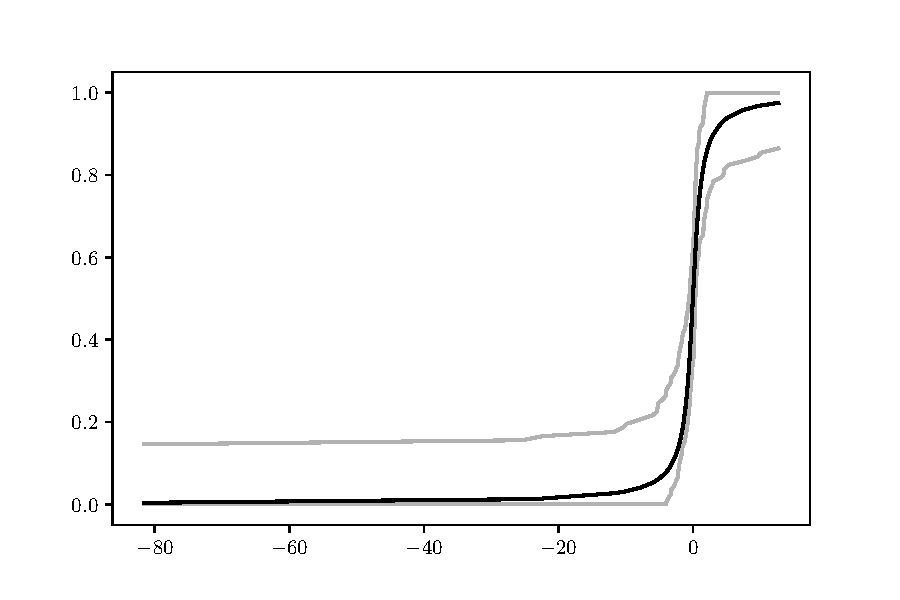
\includegraphics[scale=0.45]{../figs/max_cauchy_bands.pdf}
      \caption{Best enclosing band.}
      \label{subfig:best_band_cauchy}
  \end{subfigure}
  \caption{Confidence bands for $F$ of normal data.}
  \label{fig:bands_cauchy}
\end{figure}

\subsection*{Page 24, Exercise 7}

Let $X_{1}, \ldots, X_{n} \sim$ Bernoulli $(p)$ and let
$Y_{1}, \ldots, Y_{m} \sim$ Bernoulli $(q)$ with a $p$ = 0.5 and $q$ =
1 - $p$.

The plug-in estimator for $p$ is $\widehat{p}$ = 0.51 with a estimated
standard error $\widehat{se}$ = 0.0928 and an approximate 90 percent
confidence interval for $p$ of (0.3405, 0.6594).

The plug-in estimator for $p-q$ is $\widehat{p-q}$ = 0.5 with a
estimated standard error $\widehat{se}$ = 0.0832 and an approximate 90
percent confidence interval for $p-q$ of (0.3830, 0.6169).

The estimates above show very similar results, with very slight
differences in the intervals and the estimated standard error.

\subsection*{Page 39, Exercise 2}

The influence function is used to approximate the standard error of a
plug-in estimator. In this case, the empirical influence function was
use:

The empirical influence function is defined by
$\widehat{L}(x)=L_{\widehat{F}_{n}}(x) .$ Thus,
\[
  \widehat{L}(x)=\lim _{\epsilon \rightarrow 0}
  \frac{T\left((1-\epsilon) \widehat{F}_{n}+\epsilon
      \delta_{x}\right)-T\left(\widehat{F}_{n}\right)}{\epsilon}
\]

To estimate the the standard error, the empirical influence function,
the jackknife and the bootstrap were used. The results were: Variance
Bootstrap $v_{\text {boot }}$ = 7.5380x$10^{-17}$, Variance Jackknife
$v_{\text {jack }}$ = 0.0176, Variance Influence
$v_{\text {Influence }}$ = 0.4731 and a 95 percent studentized pivotal
bootstrap confidence interval of [0.5459189161795877,
0.5459189161795885]. This shows that the LSAT scores and GPA data are
very similar to each other, since a very close variance is observed in
the multiple test cases.


\subsection*{Page 40, Exercise 6}
The objective of this experiment is to compare the four different
confidence intervals exposed for the Bootstrap method. The Bootstrap
is performed over a sample of lognormally distributed data, taking 50
standard normal observations and making the exponentiation with the
natural base. The statistic to be evaluated is the skewness of the
data, which is well known to be positive for lognormal data. The
results are presented in Table \ref{tab:cis}.
\begin{table}[H]
  \centering
\begin{tabular}{ll}
  \hline
  \multicolumn{1}{c}{\textbf{Method}} & \multicolumn{1}{c}{\textbf{95\% C.I.}} \\ \hline
  Normal                              & (1.23, 3.41)                           \\
  Pivotal                             & (1.07, 3.22)                           \\
  Studentized                         & (1.63, 3.57)                           \\
  Percentile                          & (1.05, 3.20)                           \\ \hline
\end{tabular}
\caption{}
\label{tab:cis}
\end{table}

\subsection*{Page 40, Exercise 7}
Let
\[
  X_{1}, \ldots, X_{n} \sim t_{3}
\]

where $n=25$ and $t_{3}$ is a student's t-distribution with $\nu$ =
3. Let $\theta=T(F)=(q .75-q .25) / 1.34$. A simulation was
implemented to compare the coverage and length of the following
confidence intervals for $\theta$: Normal interval with standard error
from the bootstrap : [1.5486, 0.1564], bootstrap percentile
interval:[0.3823, 1.3026] and a normal interval with standard error
from the jackknife: [0.8141, 0.8905].

This results shows that the jackknife does not give a consistent
estimator of the variance of a quantile, showing a very short coverage
for the estimator, however, both bootstrap methods show a coverage and
length very similar to each other, with the difference that the
bootstrap percentile interval has a smaller lower bound, this is
because it is a quantile method, With a statistics that have a small
lower bound.


\subsection*{Page 40, Exercise 10}
Let $X_1, \ldots, X_n \sim \mathrm{Normal}(\mu,1)$. Let
$\theta = e^\mu$ and $\hat{\theta}=e^{\bar{x}}$ be the MLE. Create a
data set (using $\mu = 5$) consisting of $n = 100$ observations.
\begin{enumerate}[label=\alph*)]
\item Use the delta method to get the se and 95 percent confidence
  interval for $\theta.$. Use the parametric bootstrap to get the se
  and 95 percent confidence interval for $\theta.$. Use the
  nonparametric bootstrap to get the se and 95 percent confidence
  interval for $\theta.$ Compare your answers.
\item Plot a histogram of the bootstrap replications for the
  parametric and nonparametric bootstraps. These are estimates of the
  distribution of $\hat{\theta}$. The delta method also gives an
  approximation to this distribution, namely
  $\mathrm{Normal}(\hat{\theta}, \hat{se}^2)$. Compare these to the
  true sampling distribution of $\hat{\theta}$. Which approximation is
  closer to the true distribution?
\end{enumerate}
\begin{proof}
  Let's solve each item.
  \begin{enumerate}[label=\alph*)]
  \item For the delta method, it is necessary to find the influence
    function for the estimator. In first place, the plug-in
    estimator:
    \begin{align*}
      \theta &= e^\mu \\
             &= T(F) \\
             &= e^{\int u dF(u)}
    \end{align*}
    Now, the influence function:
    \begin{align*}
      L_F(x) &= \lim_{\epsilon \rightarrow 0} \frac{T\left[(1 - \epsilon)F +
               \epsilon \delta_x\right] - T(F)}{\epsilon} \\
      &= \lim_{\epsilon \rightarrow 0} \frac{e^{\int u d\left[(1 - \epsilon)F +
        \epsilon \delta_x\right]} - e^{\int u dF(u)}}{\epsilon} \\
             &= \lim_{\epsilon \rightarrow 0} \frac{e^{(1 - \epsilon)\mu + \epsilon x} - e^\mu}
               {\epsilon} \\
             &= e^\mu \lim_{\epsilon \rightarrow 0} \frac{e^{\epsilon(x - \mu)} - 1}{\epsilon}
             \quad \left[\frac{0}{0}\right]\\
             &\text{Applying L'Hopital's rule} \\
             &= e^\mu \lim_{\epsilon \rightarrow 0} \left((x - \mu) e^{\epsilon(x - \mu)}\right) \\
             &= e^\mu (x - \mu)
    \end{align*}
    Hence:
    \begin{equation*}
      \hat{L}(x) = e^{\bar{X}} (x - \mu)
    \end{equation*}

    Using the parametric and non-parametric normal bootstrap method,
    the results are found in Table \ref{tab:cis1}.
    \begin{table}[H]
      \centering
      \begin{tabular}{ll}
        \hline
        \multicolumn{1}{c}{\textbf{Method}} & \multicolumn{1}{c}{\textbf{95\% C.I.}} \\ \hline
        Delta                               & (128.52, 188.11)     \\
        Parametric                          & (127.60, 189.03)     \\
        Non-Parametric                      & (128.25, 188.38)
      \end{tabular}
      \caption{}
      \label{tab:cis1}
    \end{table}

  \item The comparison of the real distribution and the estimation
    done in the methods is shown in Figure \ref{fig:ex11}
    \begin{figure}[H]
      \centering
      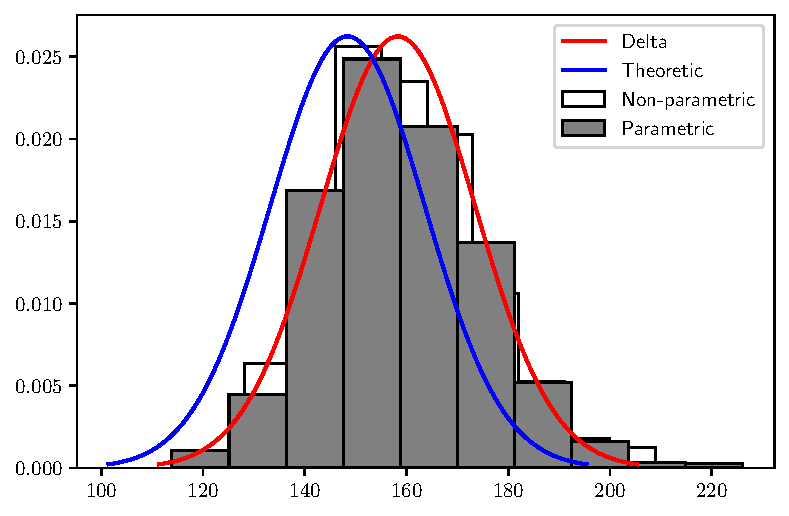
\includegraphics[scale=0.5]{../figs/delta-np.pdf}
      \caption{Comparison of distributions.}
      \label{fig:ex11}
    \end{figure}
    It is easy to see that the non-parametric bootstrap method is the
    closest one to the real distribution, as its peak does not have a
    significant bias, different to the other ones.
  \end{enumerate}
\end{proof}
\subsection*{Page 41, Exercise 11}
Let
$X_1,...,X_n\sim \mathrm{Uniform}(0,1)$, the maximum likelihood
estimator (MLE) for $\theta=1$ is
$\hat{\theta}=X_{\max}=\max\{X_1,...,X_n\}$. The distribution of
$\hat{\theta}$ is a direct consequence of the proof made in Subsection
\ref{subsec:7} and it is given by
\[
  F(t)=t^n.
\]
In Figure \ref{fig:max_density} shows the theoretical density of
$X_{\max}$ and the approximation in histograms by parametric and
nonparametric Bootstrap.
\begin{figure}[H]
  \centering
  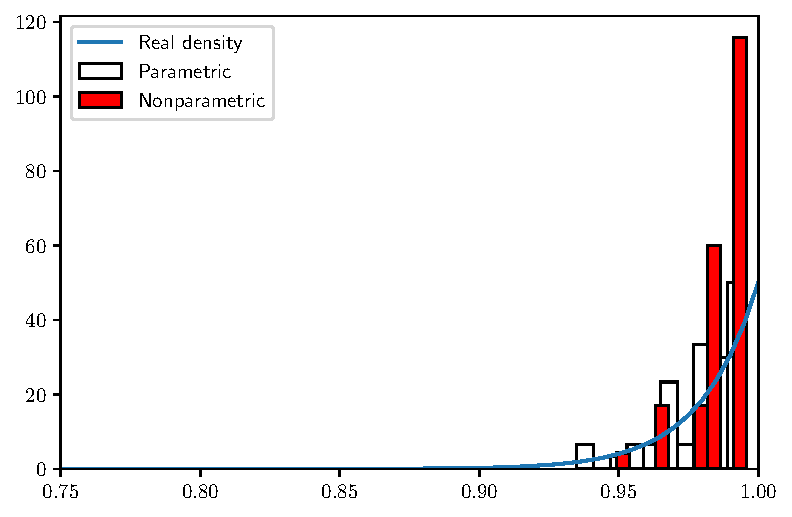
\includegraphics[scale=.7]{../figs/max_density.pdf}
  \caption{Density of $X_{\max}$, parametric and nonparametric
    histograms of $X_{\max}$.}
  \label{fig:max_density}
\end{figure}

Let $\hat{\theta}^*$ be the estimation of the parameter $\theta$ for
each Bootstrap replication. For a parametric Bootstrap, one could draw
samples from $F_{\hat{\theta}}$, instead of drawing samples from the
empirial distribuion $\hat{F}_n$. Therefore, we would draw a $N$
(number of Bootstrap iterations) new samples
$X_1^j,...,X_n^j\sim\mathrm{Uniform}(0,X_{\max})$, for
$j=1,...,N$. Clearly, $P(\hat{\theta}^*=\hat{\theta})=0$, since it is
the probability of a point on a continuous random variable, which is
obvious that it has a probability measure 0.

On the other hand, for a nonparametric Bootstrap, the procedure would
be to draw new samples from the empirical distribution, i.e. simply
draw samples with replacement from the initial sample $X_1,...,X_n$
and calculate the new estimation. In this case,
$P(\hat{\theta}^*=\hat{\theta})\approx1-(1-\frac{1}{n})^n$, since the
event $\hat{\theta}^*=\hat{\theta}$ could be interpreted as the
probability of $\hat{\theta}^*$ appearing at least once within the
$j$-th resample for the nonparametric Bootstrap.

Now, in order to calculate the true probabilty of the event
$\hat{\theta}^*=\hat{\theta}$, take the limit as
$n\rightarrow\infty$. It is well known that
$(1-\frac{1}{n})^n\rightarrow e^{-1}$ as $n\rightarrow\infty$. Then,
$P(\hat{\theta}^*=\hat{\theta})=1-e^{-1}\approx0.632$.

\printbibliography
\end{document}
